\chapter{Элементы теории парусной яхты}

\section{Требования, предъявляемые к парусной яхте.}

К уровню комфорта и оборудования на борту парусных яхт, в частности
крейсерско\-/гоночных классов, предъявляются известные требования в
соответствии с их назначением. Однако самый высокий уровень комфорта,
самые совершенные приспособления для настройки парусов, самые
современные электронные приборы для управления яхтой окажутся
бесполезными, если она не будет обладать мореходными качествами,
которые гарантируют безопасность плавания при условиях, определенных
районом плавания и назначением яхты.

Яхта должна принимать определенную нагрузку, сохраняя достаточную
высоту надводного борта, чтобы не быть залитой на волне. Она должна
противостоять давлению ветра на паруса, чтобы не быть опрокинутой
внезапно налетевшим шквалом. От яхты требуется хорошая маневренность в
тесной гавани, и послушность рулю на штормовой волне. Она должна
поддерживать, возможно, более высокую скорость при любых условиях и
быть способной идти круто к ветру. Все это и составляет важнейшие
мореходные качества: плавучесть, непотопляемость, остойчивость,
ходкость, управляемость, поведение при волнении, способность нести
паруса.

Изучение этих качеств является предметом специальной науки \--- теории
корабля. Эта наука определяет также элементы, которые составляют
отдельные мореходные качества и которые позволяют оценивать их
количественно. Наконец, теория корабля устанавливает связь между
формой корпуса судна и характеристиками его мореходных качеств.

В настоящей главе приводятся важнейшие элементы теории корабля в
приложении к парусной яхте средних размерений в объеме, необходимом
капитану при выходе в плавание.

\section{Характеристики формы корпуса яхты}

\index{характеристики формы корпуса яхты}Основными характеристиками
корпуса яхты являются его главные размерения\index{главные размерения}
и теоретический чертеж\index{теоретический чертёж}, дающий
представление об обводах корпуса.

Главными размерениями яхты являются её длина\index{главные размерения!длина},
ширина\index{главные размерения!ширина},
высота\index{главные размерения!высота борта} борта и
осадка\index{главные размерения!осадка}\index{осадка} (рис.~\ris{1}). Знание этих
величин необходимо для решения некоторых задач (плавание на
мелководье, швартовка и т.\=,д.). Различают несколько значений каждого
из этих размерений.

\begin{figure*}[htb]
   \centering
   \includegraphics[scale=1.3]{0001P.pdf}
   \caption{Главные размерения яхты}
   \label{fig:1}
\end{figure*}

\begin{description}
\item [Длина наибольшая\index{длина наибольшая}] (в проектной
  документации судов она обозначается $L$) \--- расстояние по
  горизонтали, измеренное между крайними точками по обшивке судна.
\item [Длина по конструктивной ватерлинии\index{длина по конструктивной ватерлинии}
  (\textit{КВЛ})] (\lkvl) \--- расстояние
  между крайними точками корпуса, измеренное по зеркалу воды при
  полной нагрузке судна либо при другой характерной нагрузке, например
  в состоянии обмера (см.~гл.~\ref{chap:4}).
\item [Ширина наибольшая\index{ширина наибольшая}] ($B$) \---
  измеряется в самом широком месте судна.
\item [Ширина по КВЛ\index{ширина по конструктивной ватерлинии}]
  (\bkvl) \--- наибольшая ширина, измеренная в плоскости ватерлинии.
\item [Высота надводного борта\index{высота надводного борта}] ($F$)
  \--- измеряется от ватерлинии до верхней кромки палубного настила у
  борта. Различают минимальный надводный борт \cidx{F}{М}, надводный
  борт в носу \cidx{F}{А} (измеряется по отвесу, опущенному из самой
  крайней точки форштевня) и надводный борт в корме \cidx{F}{К} (по
  отвесу, опущенному из крайней кормовой точки пересечения линии
  палубы с поверхностью транца).
\item [Осадка средняя\index{осадка!средняя}] (\tsr) \--- углубление
  судна, измеренное в средней части \--- на миделе \--- от ватерлинии
  до нижней кромки фальшкиля. На яхтах с длинной килевой линией
  измеряют еще максимальную осадку \--- от ватерлинии до самой нижней
  точки киля, обычно расположенной вблизи пятки руля.
\item [Полная высота борта на миделе\index{полная высота борта на миделе}]
  ($H$) измеряется от верхней плоскости балластного
  фальшкиля до верхней кромки палубного настила у борта. Вместе с $L$
  и $B$ высота борта используется в правилах постройки и классификации
  яхт в качестве параметра для назначения размеров поперечного сечения
  деталей набора корпуса, элементов якорного устройства и т.\=,п.
\end{description}

Кроме главных размерений корпуса существуют еще габаритные
размеры\index{габаритные размеры}, например длина вместе с бушпритом,
высота от нижней точки киля до верхней точки надстройки, ширина вместе
с выступающими снаружи обшивки буртиками или привальным брусьями и
т.\=,п.

Главные размерения яхты определяются из условий обеспечения требуемых
мореходных качеств, внутреннего расположения жилых и служебных
помещений, часто с целью получить определенный гоночный балл или
класс. Они являются одними из основных количественных элементов,
характеризующих эксплуатационные качества судна \--- его мореходность,
вместимость и обитаемость.

Кроме абсолютных цифр судостроители и моряки часто оперируют
безразмерными характеристиками \--- соотношениями главных
размерений. Наиболее употребительными являются следующие.

\begin{description}
\item [Отношение длины по ватерлинии к ширине\index{отношение!длины по ватерлинии к ширине}]
  $\lkvl / \bkvl$ \--- характеризует ходкость
  судна (чем больше $ \lkvl / \bkvl$, тем легче на ходу, быстроходнее
  судно) и остойчивость (чем меньше $ \lkvl / \bkvl$, тем остойчивее
  яхта). У современных крейсерско-гоночных яхт, построенных по
  правилам IOR, $L/B = 2,5 \motdo 5,0$, у крейсерских швертботов
  $L/B = 2,8 \motdo 3,8$.
\item [Отношение ширины по КВЛ к осадке\index{отношение!ширины по КВЛ к осадке}]
  $\bkvl / \tsr$ \--- характеризует ходкость,
  остойчивость и мореходность. Чем больше $\bkvl / \tsr$, тем
  остойчивее судно, однако его способность сохранять скорость при
  волнении оказывается ниже, чем у более узкой и глубокосидящей
  яхты. Яхты с классическими обводами корпусов имели
  $\bkvl / \tsr = 1,2 \motdo 1,6$; у современных крейсерско\-/гоночных
  яхт $\bkvl / \tsr = 1,8$. Для современных килевых яхт с выраженным
  плавниковым килем более характерно отношение $\bkvl / \cidx{T}{к}$,
  т.\=,е. ширины по КВЛ к осадке корпуса (без киля).
\item [Отношение наибольшей длины к высоте борта\index{отношение!наибольшей длины к высоте борта}]
  $L/H$ \--- характеризует
  прочность и жесткость корпуса. Чем отношение меньше, тем большей
  продольной жесткостью обладает корпус, тем меньше он деформируется
  на волне и от тяги штагов.
\end{description}

Теоретический чертеж яхты представляет сложную криволинейную наружную
поверхность корпуса в виде проекций на три взаимно перпендикулярные
плоскости. На этих проекциях изображаются следы пересечения наружной
обшивки с секущими плоскостями, положение которых определяется в
соответствии с установившимися в судостроении правилами. Три плоскости
\--- диаметральная, основная и плоскость мидель-шпангоута являются
базовыми плоскостями для построения теоретического чертежа и для
постройки судна; они используются в качестве координатных плоскостей,
от которых отсчитывают все размеры при последующей модернизации яхты.

\begin{description}
\item [Диаметральная плоскость\index{диаметральная плоскость}]
  (\textit{ДП}) \--- вертикальная продольная плоскость симметрии,
  разделяющая корпус яхты на правую и левую половины.
\item [Основная плоскость\index{основная плоскость}] (\textit{ОП})
  \--- горизонтальная плоскость, проходящая через самую нижнюю точку
  киля. Линия пересечения основной плоскости с \textit{ДП} называется
  основной линией (\textit{ОЛ}).
\item [Плоскость мидель-шпангоута\index{плоскость мидель-шпангоута}]
  (\textbf{миделя}\index{мидель}) \--- вертикальная поперечная
  плоскость, проходящая посередине длины яхты по КВЛ. Эту плоскость
  обозначают значком миделя \--- \midelsign. При оценке формы корпуса
  принято считать миделем самый большой по площади погруженной части
  шпангоут.
\end{description}

Три проекции теоретического чертежа получаются сечением корпуса
плоскостями, параллельными перечисленным трем базовым
плоскостям. Боковая проекция\index{проекция!боковая} (\textbf{<<бок>>}) образуется в
результате сечения корпуса равноотстоящими друг от друга плоскостями,
параллельными \textit{ДП}. Показанные на ней кривые линии сечений
называются \textbf{батоксами}\index{проекция!батокс}. Аналогичным образом получаются две
другие проекции \--- \textbf{<<полуширота>>}\index{проекция!полуширота} и
\textbf{<<корпус>>}. Первая образуется сечениями корпуса плоскостями,
параллельными \textit{ОП} \--- \textbf{ватерлиниями}\index{проекция!ватерлиния}, вторая \---
сечением корпуса плоскостями, параллельными миделю \---
\textbf{шпангоутами}\index{проекция!шпангоут}. На <<боку>> и <<полушироте>> шпангоуты
изображаются в виде прямых линий; на <<корпусе>> они
криволинейные. Ватерлинии выглядят в виде прямых на <<боку>> и
<<корпусе>>, а батоксы \--- на <<полушироте>> и <<корпусе>>
(рис.~\ris{2}). Прямые линии на каждой проекции образуют сетку
теоретического чертежа.

\begin{figure*}[htb]
   \centering
   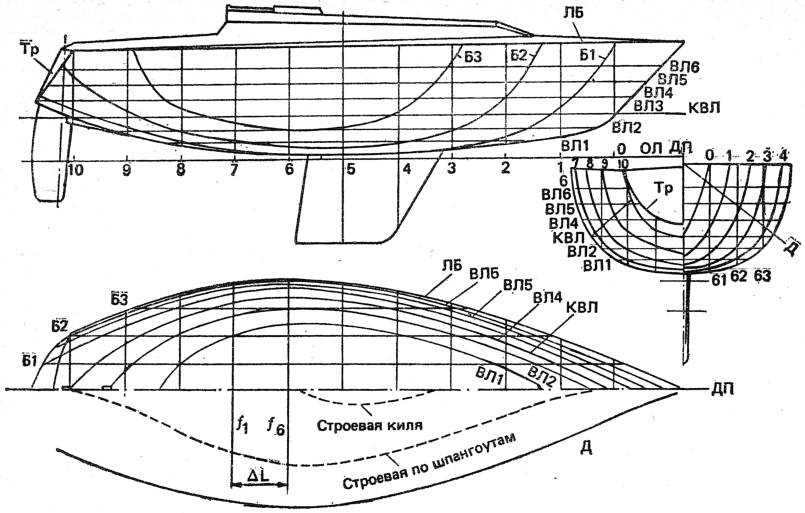
\includegraphics[scale=1.3]{0002P.pdf}
   \caption{Теоретический чертеж яхты <<Симфония>> (конструктор Филипп Брайан, Франция)}
   \label{fig:2}
   \centering{}
   \small  
   Длина наибольшая \--- 9,5~м;
   ширина наибольшая \--- 3,25~м;
   надводный борт минимальный \--- 1,02~м;
   осадка \--- 1,88~м;
   водоизмещение полное \--- 5,14~т.
   1\==10 \--- шпангоуты,
   Тр \--- транец,
   ЛБ \--- линия борта,
   Б1\==Б3 \--- батоксы,
   ВЛ1\==ВЛ6 \--- ватерлинии,
   Д \--- диагональ (рыбина).
\end{figure*}

На теоретическом чертеже кроме упомянутых линий батоксов, шпангоутов и
ватерлиний изображают очертания плавниковых килей, рулей, транца,
фальшборта и т.\=,п. Так как корпус симметричен относительно
\textit{ДП}, то на полушироте изображают ватерлинии только левого
борта; на проекции <<Бок>> по правую сторону от линии \textit{ДП}
вычерчивают обводы носовых шпангоутов, а по левую \--- обводы
кормовых.

Все линии теоретического чертежа должны быть согласованы. Это значит,
что любая точка на поверхности корпуса должна отстоять на равных
расстояниях, например от \textit{ДП} на всех трех проекциях. При
согласовании линий конструктор обычно проверяет положение точек
пересечения кривых линий с прямыми линиями сетки. Для дополнительного
согласования обводов корпуса на теоретическом чертеже проводят рыбины
или диагонали \--- следы сечения корпуса продольными, наклонными к
\textit{ДП} плоскостями, проведенными через характерные точки на
проекции <<корпус>> \--- скулу, вогнутость при киле и
т.\=,п. Диагонали проводятся только на <<корпусе>>, в виде прямых
линий, и на полушироте вниз от \textit{ДП}, где они имеют вид плавных
кривых линий.

Опытному глазу каждая из линий теоретического чертежа может многое
сказать о качествах судна. Например, плавные стройные ватерлинии с
острым входом в носу и не слишком крутой кривизной в корме
благоприятны для хорошего обтекания корпуса водой, как и диагонали
аналогичного вида. Батоксы с плавным и пологим \--- под углом
$15 \motdo 20\gr$ к \textit{КВЛ} выходом над ватерлинией также важны
для плавного, без завихрений, обтекания корпуса. Шпангоуты с явно
выраженной скулой и переходом днища в борта по малому радиусу
свидетельствуют о высокой начальной остойчивости яхты. В носовой части
V-образные шпангоуты с острой вершиной при киле и плавным расширением
к палубе важны для сохранения скорости на взволнованном море и
незаливаемости палубы.

Существенное влияние на обводы корпуса оказывают \textbf{Правила обмера},
по которым строится яхта. Так, в 70-х годах в результате
введенного в правила обмера IOR, замера глубины трюма (расстояний от
\textit{КВЛ} до внутренней поверхности обшивки) на миделе в трех
местах по ширине яхты появились суда с трапециевидными
шпангоутами. Эти же Правила дали жизнь принципиально новым обводам
корпусов \--- с короткими свесами оконечностей, <<обратным>> наклоном
транца, высоким надводным бортом и плавниковым килем, которые
значительно отличаются от классических яхтенных обводов,
господствовавших до конца 60-х годов.

Важнейшей характеристикой яхты является её \textbf{объемное водоизмещение}\index{водоизмещение!объемное}
$V$, т.\=,е. объем воды, вытесняемый яхтой при её погружении по \textit{КВЛ}.
Объемное водоизмещение яхты вместе с её главными размерениями позволяет судить
о величине судна, его вместимости и потенциальных мореходных качествах. При
сравнении яхт часто пользуются безразмерной характеристикой \---
\textbf{коэффициентом полноты водоизмещения}\index{коэффициент!полноты!водоизмещения}
или \textbf{коэффициентом общей полноты}\index{{коэффициент!полноты!общей}}
$\delta$, связывающим линейные размеры корпуса с его погруженным объемом.
Этот коэффициент определяется как отношение объемного водоизмещения к
объему параллелепипеда, имеющего стороны, равные \lkvl, \bkvl и \tsr (рис.~\ris{3}): 

\begin{equation}
  \delta = \frac{V}{(\lkvl \cdot \bkvl \cdot  \tsr)}
\end{equation}

\begin{figure}[htb]
   \centering
   \includegraphics[scale=1.1]{0003P.pdf}
   \caption{Коэффициенты полноты}
   \label{fig:3}
   \centering{}\small $\delta$ \--- водоизмещения; $\alpha$ \--- ватерлинии; $\varphi$ \--- продольной полноты; $\beta$ \--- полноты мидель-шпангоута
\end{figure}

Чем меньше коэффициент общей полноты, тем более острые обводы имеет
яхта, тем она быстроходнее. С другой стороны, при уменьшении $\delta$
соответственно уменьшается и полезный объем корпуса ниже ватерлинии,
что вызывает необходимость для размещения кают достаточной высоты
увеличивать высоту борта или делать более высокие надстройки. Парусные
яхты относят к наименее полным судам. Коэффициент общей полноты для
крейсерско-гоночных яхт составляет $\delta = 0,15 \motdo 0,22$, для
крейсерских швертботов $\delta = 0,26 \motdo 0,35$. Корпуса шхерных
крейсеров имели $\delta = 0,12 \motdo 0,15$, в то время как для
большинства грузовых коммерческих судов характерна величина
$\delta = 0,82$.

К числу безразмерных коэффициентов, характеризующих форму корпуса
яхты, относятся также \textbf{коэффициенты полноты площадей ватерлинии}
\index{коэффициент!полноты!площади!ватерлинии} $\alpha$ и
\textbf{мидель-шпангоута}\index{коэффициент!полноты!площади!мидель-шпангоута}
$\beta$. Первый представляет собой отношение площади ватерлинии $S$ к
прямоугольнику со сторонами \lkvl и \bkvl:

\begin{equation}
  \alpha = \frac{S}{\lkvl \cdot \bkvl} \quad ;
\end{equation}

второй \--- отношение площади погруженной части миделя \midelsign к
прямоугольнику, стороны которого равны \bkvl и \tsr:

\begin{equation}
\beta =  \frac{\midelsign}{\bkvl \cdot \tsr}
\end{equation}

Коэффициент $\alpha$, равный для большинства крейсерских яхт 0,70\otdo
0,72, для швертботов 0,60\otdo 0,67, показывает, насколько заострена
\textit{КВЛ} в оконечностях, и какую роль в начальной остойчивости
яхты играет форма её корпуса. С увеличением полноты ватерлинии
повышается остойчивость, но несколько ухудшается обтекаемость корпуса
и его ходкость на волне, особенно при большой осадке.

\textbf{Коэффициент продольной полноты}\index{коэффициент!продольной полноты}
(или \textbf{призматический}\index{коэффициент!призматически}) $\varphi$,
который представляет собой отношение объемного водоизмещения к объему
призмы, имеющей основанием погруженную часть миделя, а высотой длину
яхты по КВЛ служит для оценки сопротивления воды движению яхт:

\begin{equation}
\varphi = \frac{V}{\midelsign \cdot \lkvl}
\end{equation}

Призматический коэффициент, характеризуя распределение погруженного
объема корпуса по длине, оказывает существенное влияние на ту часть
энергии ветра, которая затрачивается на преодоление волнового
сопротивления корпуса. Оптимальная величина $\varphi$ зависит от того,
на какую скорость рассчитывается яхта. Если речь идет об очень
быстроходных судах, то $\varphi$ принимается близким к
$\varphi \approx 0,62$. Для яхт проектируемых на слабые ветра,
$\varphi = 0,52 \motdo 0,53$.

\section{Плавучесть, осадка и дифферент}\index{плавучесть}\index{осадка}\index{дифферент}

\textbf{Плавучесть}\index{плавучесть} \--- способность судна держаться
на плаву, имея заданную осадку при определенной нагрузке. Это качество
должно сохраняться в любых обстоятельствах эксплуатации яхты.

На погруженную в воду поверхность судна при его неподвижном состоянии
в каждой точке действуют силы гидростатического давления воды,
направленные перпендикулярно поверхности. Все эти силы можно привести
к одной силе плавучести, направленной вверх и приложенной в центре
тяжести погруженного объема \--- \textbf{центре величины}\index{центр!величины},
\textit{ЦВ}. Согласно известному закону Архимеда, сила
плавучести равна массе воды, вытесненной судном.

Кроме давления воды на корпус судна действуют силы тяжести, которые
также могут быть приведены к одной равнодействующей силе $D$,
направленной вниз и приложенной в \textbf{центре тяжести}\index{центр!тяжести},
\textit{ЦТ}
судна. Для того чтобы судно плавало в состоянии равновесия,
необходимо, чтобы сила плавучести и сила тяжести были равны и
располагались на одной вертикали:

\begin{gather}
  D = \gamma \cdot V \,;\  \cidx{x}{д} = \cidx{x}{с}
\end{gather}

где $\gamma$ \--- плотность воды, $\mbox{т}/\mbox{м}^3$; $V$ \---
объемное водоизмещение, $\mbox{м}^3$; $D$ \--- масса судна или
массовое водоизмещение, т; \cidx{x}{д} \--- отстояние центра тяжести,
\textit{ЦТ}, от плоскости миделя, м; \cidx{x}{с} \--- отстояние центра
величины, \textit{ЦВ} от плоскости миделя, м.

В зависимости от плотности воды, в которой плавает яхта, её объемное
водоизмещение может изменяться, хотя масса судна остается
постоянной. В пресной воде, плотность которой близка к единице, для
поддержания судна определенной массы требуется больший погруженный
объем V, чем в соленой воде, плотность которой колеблется от
$\gamma = 1,010 \motdo 1,015 \, \mbox{т}/\mbox{м}^3$ в Балтийском море
до $1,023 \motdo 1,028 \, \mbox{т}/\mbox{м}^3$ в океане. Изменение
объемного водоизмещения при переходе яхты из пресной воды
($\gamma = 1,00$) в морскую и наоборот происходит за счет изменения
осадки. Величина этого изменения невелика \--- менее 1\,\% осадки и на
эксплуатационных качествах яхты практически не сказывается. Однако
влияние солености на осадку следует учитывать при обмере яхты и
вычислении её гоночного балла.

Знание главных размерений яхты и её коэффициентов полноты позволяет
капитану выполнять некоторые элементарные расчеты приближенных
значений водоизмещения, изменения осадки при приеме груза относительно
небольшой величины.

Водоизмещение\index{водоизмещение}:
\begin{equation}
D = \gamma \cdot \delta \cdot \lkvl \cdot \bkvl \cdot \tsr, \mbox{т.} 
\end{equation}

Груз, изменяющий осадку на 1 см:

\begin{equation}
  p = 0,01 \cdot \gamma \cdot \alpha \cdot \lkvl \cdot \bkvl, \mbox{т.}
\end{equation}

\begin{table*}[htb]
  \centering{}
  \begin{tabular}{p{0.5\textwidth}|c}
    \toprule
    Наименование раздела массовой нагрузки & Массовое водоизмещение, \,\% \\
    \midrule
    Корпус & 30--43 \\
    \midrule
    Фальшкиль & 30--45 \\
    \midrule
    Дельные вещи в корпусе и на палубе & 2--4,5 \\
    \midrule
    Оборудование помещений & 3--7 \\
    \midrule
    Рангоут, такелаж и паруса & 4--7 \\
    \midrule
    Двигатель с трубопроводами и электрооборудованием & 0--7 \\ 
    \midrule
    Системы с трубопроводами и цистернами & 2--4 \\
    \midrule
    Полезная нагрузка: экипаж с багажом, запасы пресной воды, провизии и топлива & 6--8 \\
    \bottomrule
    Массовое водоизмещение & $D = 100\,\%$ \\
  \end{tabular}
  \caption{Примерное распределение массового водоимещения между разделами нагрузки для крейсерско-гоночных яхт длиной 10\--14 метров}
  \label{tab:1}
\end{table*}

Если при проектировании или постройке яхты окажется, что её масса
превышает водоизмещение по \textit{КВЛ}, а \textit{ЦТ} смещен в нос
или корму от \textit{ЦВ}, то при спуске на воду она погрузится глубже
конструктивной ватерлинии и получит наклон \---
\textbf{дифферент}\index{дифферент} на нос или на корму. При
продольном наклонении в воду погружается дополнительный объем корпуса
в носу или корме и в ту же сторону смещается точка приложения
равнодействующей сил плавучести (\textit{ЦВ}) до того момента, пока
вновь не будет достигнуто условие плавания в состоянии равновесия
т.\=,е. $\cidx{x}{д} = \cidx{x}{с}$.

И увеличение осадки, и дифферент нежелательны, так как обводы
ватерлиний яхты могут существенно отличаться от тех, что были
предусмотрены её посадкой по проектной \textit{КВЛ}. Чтобы этого не
случилось, после выбора главных размерений конструктор должен хотя бы
приблизительно оценить массу будущей яхты. Для этого выполняется
предварительный расчет массовой нагрузки по основным разделам: корпус;
дельные вещи и палубное оборудование; оборудование внутренних
помещений; рангоут, такелаж и паруса; двигатель с трубопроводами,
гребным валом и электрооборудованием; системы с трубопроводами,
цистернами; полезная нагрузка \--- экипаж, запасы пресной воды и
провизии топливо для двигателя, снабжение; балластный
фальшкиль. Примерное соотношение этих составляющих массовой нагрузки
дано в табл.~\ref{tab:1}, а сумма их должна быть равна массово
водоизмещению яхты по \textit{КВЛ}.

Существенное влияние на дифферент яхты оказывают переменные массы \---
топливо и вода в цистернах, которые расходуются в течение плавания, а
также экипаж, имеющий возможность перемещаться по яхте. Поэтому
цистерны для жидкостей стараются располагать вблизи общего ЦТ яхты, а
экипаж во время гонки рассредоточивать на палубе и в помещениях, не
допуская его скопления в кормовом кокпите, где масса людей создает
значительный дифферентующий момент на корму.

\section{Непотопляемость}

Способность судна оставаться на плаву и сохранять свои мореходные
качества в случае получения пробоины в обшивке или затопления через
палубные отверстия называется
\textbf{непотопляемостью}\index{непотопляемость}. Это свойство в
первую очередь определяется запасом плавучести судна \--- его
надводным объемом от \textit{КВЛ} до палубы. Чем выше надводный борт,
тем больше запас плавучести, тем большее количество воды может влиться
внутрь яхты, прежде чем она затонет.

Непотопляемость безбалластных швертботов и небольших яхт обеспечить
сравнительно несложно. Благодаря легкой конструкции корпуса разность
между массой яхты и силой поддержания в аварийном состоянии
невелика. Требуется лишь небольшой дополнительный запас плавучести в
виде междудонного пространства, бортовых отсеков плавучести,
герметичных отсеков в носу и корме, под кокпитом. Для большей
надежности эти отсеки заполняют легким пенистым пластиком, не
впитывающим воду. Объем отсеков плавучести или блоков пенопласта
рассчитывают так, чтобы при заполнении водой яхта держалась на плаву с
надводным бортом около 10\,см и по возможности на ровном киле. Чтобы
она сохраняла свою способность сопротивляться крену и дифференту,
отсеки плавучести размещают в оконечностях корпуса и по бортам.

Обеспечить непотопляемость крупной яхты, снабженной фальшкилем массой
40\--50\,\% её водоизмещения и имеющей большой объем внутренних
помещений, практически невозможно. В данном случае помогло бы деление
корпуса поперечными водонепроницаемыми переборками на несколько
отсеков. Однако глухие переборки создают большие неудобства для
обитаемости яхт, а при устройстве дверей переборки теряют
смысл. Поэтому даже на больших яхтах устанавливают две
водонепроницаемые переборки \--- форпиковую (вблизи носового конца
\textit{КВЛ}) и ахтерпиковую (в районе кокпита), ограничивающие доступ
воды внутрь при получении пробоины в оконечностях.

Опыт, однако, показывает, что в море от пробоин при столкновениях яхты
гибнут сравнительно редко. Гораздо большую опасность представляет
негерметичность закрытий палубных люков, разбитые иллюминаторы. Именно
это стало причиной гибели пяти яхт в трагической Фастнетской гонке
1979\,г. у берегов Ирландии. На этих яхтах (так же как и еще на 98 из
234 участвовавших в гонке судов) причиной попадания больших масс воды
внутрь корпуса были ненадежные закрытия входных люков в стенках
рубок. Традиционные задвижные щитки выскакивали из своих пазов при
опрокидывании яхт, оказывались смытыми за борт или затерявшимися
внутри яхт.

Современная практика требует, чтобы яхта, положенная парусами на воду,
не могла быть залита через открытые люки. Входные люки предписывается
оборудовать дверцами на прочных петлях, открываемыми обязательно
наружу. Все иллюминаторы и светлые люки должны снабжаться защитными
щитками, которые в штормовых условиях устанавливаются снаружи. Все
отверстия в корпусе для забора забортной воды или выпуска сточных вод,
воды из системы охлаждения двигателя и т.\=,п. снабжаются надежными
запорными вентилями и клапанами, а осушительная система должна иметь
достаточную производительность.

Современная крейсерско-гоночная яхта обладает большой живучестью,
т.\=,е. способностью оставаться при аварии на плаву и перемещаться в
нужном направлении. В упомянутой Фастнетской гонке на гребнях крутых
волн опрокинулось 77 яхт, многие из которых совершили полный оборот на
360\gr. Несмотря на повреждения и большие массы воды, попавшие внутрь
яхт, большинство из них были приведены в порты-убежища своими
экипажами. Экипажи шести яхт, посчитавшие положение критическим,
покинули их на надувных спасательных плотах, которые в тех условиях
оказались недостаточно надежными. В результате погибло семь человек. В
то же время только две из покинутых шести яхт действительно
утонули. Четыре судна, несмотря на жестокий шторм, остались на плаву и
были впоследствии обнаружены в море и отбуксированы в гавани.

\section{Силы, действующие на корпус и паруса яхты}

\begin{figure}[htb]
  \centering\includegraphics[scale=0.9]{0004P.pdf}
  \caption{\centering{} Схема сил, действующих на корпус и паруса яхты}
  \label{fig:4}
\end{figure}

До сих пор мы рассматривали действие на яхту только двух сил \--- силы
плавучести\index{сила!плавучесть} и силы веса\index{сила!вес},
предполагая, что она находится в равновесии состоянии покоя. Но
поскольку для движения вперед на яхте используются паруса, на судно
действует сложная система сил. Схематически она представлена на
рис.~\ris{4}, где рассматривается наиболее типичный случай движения
яхты в бейдевинд.

При обтекании парусов воздушным потоком \--- ветром \--- на них
создается результирующая \textbf{аэродинамическая
  сила}\index{сила!аэродинамическая} \textbf{А}, направленная примерно
перпендикулярно поверхности паруса и приложенная в центре парусности
(\textit{ЦП})\index{центр!парусности} высоко над поверхностью
воды. Согласно третьему закону механики, при установившемся движении
тела по прямой каждой силе, приложенной к телу, в данном случае \--- к
парусам, связанным с корпусом яхты через мачту, стоячий такелаж и
шкоты, должна противодействовать равная ей по величине и
противоположно направленная сила. На яхте \--- это результирующая
\textbf{гидродинамическая сила}\index{сила!гидродинамическая}
\textbf{Н}, приложенная к подводной части корпуса. Таким образом,
между этими силами существует известное расстояние \--- плечо,
вследствие чего образуется момент пары сил.

И аэро- и гидродинамическая силы оказываются ориентированными не в
плоскости, а в пространстве, поэтому при изучении механики движения
яхты рассматривают проекции этих сил на главные координатные
плоскости. Имея в виду упомянутый третий закон Ньютона, выпишем
попарно все составляющие аэродинамической силы и соответствующие им
гидродинамические реакции (см. таб.~\ref{tab:1-1}).

\begin{table*}[htb]
  \begin{tabular}{c|p{0.3\textwidth}|c|p{0.3\textwidth}}
    \toprule
    \shortstack[c]{Сила\\Момент} & \shortstack[c]{Описание\\\ } & \shortstack[c]{Сила\\Момент} & \shortstack[c]{Описание\\\ } \\
    \midrule
    $\ve{A}$ & Проекция аэродинамической результирующей силы\index{сила!аэродинамическая!проекция} & 
    $\ve{H}$ & Проекция гидродинамической результирующей силы\index{сила!гидродинамическая!проекция} \\
    $\ve{T}$ & Сила тяги, движущая яхту вперед\index{сила!тяги} &
    $\ve{R}$ & Сила сопротивления воды движению яхты\index{сила!сопротивление воды} \\
    $\vidx{F}{Д}$ & Кренящая сила или сила дрейфа\index{сила!кренящая}\index{сила!дрейф} &
    $\vidx{R}{Д}$ & Боковая сила или сила сопротивления дрейфу\index{сила!сопротивление дрейфу}\index{сила!боковая} \\
    $\vidx{F}{В}$ & Вертикальная (аэродинамическая) сила\index{сила!аэродинамическая!вертикальная} &
    $\vidx{H}{В}$ & Вертикальная гидродинамическая сила\index{сила!гидродинамическая!вертикальная} \\
    $\ve D$ & Сила веса яхты\index{сила!вес} &
    $\gammaV$ & Сила плавучести\index{сила!плавучесть} \\
    $\ve{M}_D$ & Дифферентующий момент\index{момент!дифферентующий} &
    $\ve{M}_Z$ & Момент сопротивления дифференту\index{момент!сопротивления дифференту} \\
    $\vidx{M}{КР}$ & Кренящий момент\index{момент!кренящий} &
    $\vidx{M}{В}$ & Восстанавливающий момент\index{момент!восстанавливающий} \\
    $\vidx{M}{П}$ & Приводящий к ветру момент\index{момент!приводящий к ветру} &
    $\vidx{M}{У}$ & Уваливающий момент\index{момент!уваливающий} \\
    \bottomrule
  \end{tabular}
  \caption{Составляющие аэродинамической силы и соответствующие им гидродинамические реакции}
  \label{tab:1-1}
\end{table*}

Для того чтобы яхта устойчиво шла по курсу, каждая пара сил и каждая
пара моментов сил должны быть равны друг другу. Например, сила дрейфа
\vidx{F}{Д}, и сила сопротивления дрейфу \vidx{R}{Д} создают кренящий
момент \vidx{M}{КР}, который должен быть уравновешен восстанавливающим
моментом \vidx{M}{В} или моментом поперечной остойчивости. \vidx{M}{В}
образуется благодаря действию сил веса \ve{D} и плавучести яхты \ve V,
действующих на плече $l$. Эти же силы веса и плавучести образуют
момент сопротивления дифференту или момент продольной остойчивости
$\ve{M}_l$, равный по величине и противодействующий дифферентующему
моменту $\ve M_D$. Слагаемыми последнего являются моменты пар сил
$\ve T - \ve R$ и $\vidx{F}{В} - \vidx{H}{В}$.

В приведенную схему действия сил существенные поправки вносит,
особенно на легких яхтах, экипаж. Перемещаясь на наветренный борт или
по длине яхты, экипаж своим весом эффективно откренивает судно или
противодействует его дифференту на нос. В создании уваливающего
момента \vidx{M}{У} решающая роль принадлежит соответствующему
отклонению руля.

Аэродинамическая боковая сила \vidx{F}{Д}, кроме крена вызывает
боковой снос \--- дрейф\index{дрейф}\index{снос!боковой}, поэтому яхта
движется не строго по \textit{ДП}, а с небольшим углом дрейфа
$\lambda$. Именно это обстоятельство обусловливает образование на киле
яхты силы сопротивления дрейфу \vidx{R}{Д}, которая по своей природе
аналогична подъемной силе, возникающей на крыле самолета,
располагаемом под углом атаки к набегающему потоку. Аналогично крылу
работает на курсе бейдевинд и парус, для которого углом атаки является
угол между хордой паруса и направлением вымпельного ветра. Таким
образом, в современной теории корабля парусная яхта рассматривается
как симбиоз двух крыльев: корпуса, движущегося в воде, и паруса, на
который воздействует вымпельный ветер.

\section{Остойчивость}

Как мы уже говорили, яхта подвержена действию сил и моментов сил,
стремящихся наклонить её в поперечном и продольном
направлениях. Способность судна противостоять действию этих сил и
возвращаться в прямое положение после прекращения их действия
называется \textbf{остойчивостью}\index{остойчивость}. Наиболее важной
для яхты является \textbf{поперечная остойчивость}
\index{остойчивость!поперечная}.

\begin{figure}[htb]
   \centering
   \includegraphics[scale=1.1]{0005P.pdf}
   \caption{Остойчивость килевой яхты}
   \label{fig:5}
   \centering{}\small Плечо остойчивости $l = \cidx{l}{Ф} - \cidx{l}{В}$
\end{figure}

Когда яхта плавает без крена, то силы тяжести и плавучести,
приложенные соответственно в \textit{ЦТ} и \textit{ЦВ}, действуют по
одной вертикали. Если при крене экипаж либо другие составляющие
массовой нагрузки не перемещаются, то при любом отклонении \textit{ЦТ}
сохраняет свое первоначальное положение в \textit{ДП} (точка $G$ на
рис.~\ris{5}), вращаясь вместе с судном. В то же время вследствие
изменившейся формы подводной части корпуса \textit{ЦВ} смещается из
точки $C_0$ в сторону накрененного борта до положения $C_1$. Благодаря
этому возникает момент пары сил \ve D и \gammaV с плечом $l$, равным
горизонтальному расстоянию между \textit{ЦТ} и новым \textit{ЦВ}
яхты. Этот момент стремится возвратить яхту в прямое положение и
потому называется \textbf{восстанавливающим}
\index{момент!восстанавливающий}.

При крене ЦВ перемещается по кривой траектории $C_0C_1$, радиус
кривизны $r$ которой называется
\textbf{поперечным метацентрическим радиусом}\index{метацентр!радиус поперечный},
а соответствующий ему центр кривизны $M$ \---
\textbf{поперечным метацентром}\index{метацентр!поперечный}. Величина радиуса $r$ и соответственно
форма кривой $C_0C_1$ зависят от обводов корпуса. В общем случае при
увеличении крена метацентрический радиус уменьшается, так как его
величина пропорциональна четвертой степени ширины ватерлинии.

Очевидно, что плечо восстанавливающего момента зависит от расстояния
$GM$ \--- возвышения метацентра над центром тяжести: чем оно меньше,
тем соответственно меньше при крене и плечо $l$. На самой начальной
стадии наклона величины $GM$ или $h$ рассматривается судостроителями
как мера остойчивости судна и называется
\textbf{начальной поперечной метацентрической высотой}
\index{метацентр!высота поперечная}.
Чем больше $h$, тем необходима большая
кренящая сила, чтобы наклонить яхту на какой-либо определенный угол
крена, тем остойчивее судно. На крейсерско\-/гоночных яхтах
метацентрическая высота составляет обычно 0,75\otdo 1,2\,м; на
крейсерских швертботах \--- 0,6\otdo 0,8\,м.

По треугольнику $GMN$ легко установить, что восстанавливающее плечо: $l = G \cdot N = h \cdot \sin \Theta$

Восстанавливающий момент\index{момент!восстанавливающий}, учитывая равенство \gammaV и \ve D, равен:

\begin{equation}
  \cidx{M}{В} = D \cdot h \cdot \sin \Theta
\end{equation}

Таким образом, несмотря на то, что метацентрическая высота изменяется
в довольно узких пределах для яхт различных размерений, величина
восстанавливающего момента прямо пропорциональна водоизмещению яхты,
следовательно, более тяжелое судно оказывается в состоянии выдержать
кренящий момент большей величины.

Восстанавливающее плечо можно представить как разность двух расстояний
(см. рис.~\ris{5}): \cidx{l}{Ф} \--- плеча остойчивости формы\index{плечо!остойчивость!форма} и
\cidx{l}{В} \--- плеча остойчивости веса\index{плечо!остойчивость!вес}. Нетрудно установить
физический смысл этих величин, так как \cidx{l}{В} определяется
отклонением при крене линии действия силы веса от первоначального
положения точно над $C_0$, а \cidx{l}{Ф} \--- смещением на
подветренный борт центра величины погруженного объема
корпуса. Рассматривая действие сил \ve D и \gammaV относительно $C_0$,
можно заметить, что сила веса \ve D стремится накренить яхту еще
больше, а сила \gammaV, наоборот \--- выпрямить судно.

\begin{figure}[htb]
  \centering
  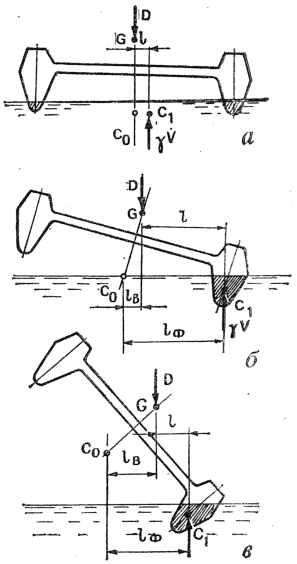
\includegraphics[scale=1.2]{0006P.pdf}
  \caption{Остойчивость катамарана}
  \label{fig:6}
  \small
  \centering{}
  \textit{а} \--- на малых углах крена;
  \textit{б} \--- в момент выхода наветренного корпуса из воды;
  \textit{в} \--- на больших углах крена
\end{figure}

По треугольнику $C_0GK$ можно найти, что
$\cidx{l}{В} = G \cdot K = C_0 \cdot G \cdot \sin \Theta$, где
$C_0 \cdot G$ \--- возвышение \textit{ЦТ} над \textit{ЦВ} в прямом
положении яхты. Таким образом, для того чтобы уменьшить отрицательное
действие сил веса, необходимо по возможности понизить \textit{ЦТ}
яхты. В идеальном случае \textit{ЦТ} должен бы расположиться ниже
\textit{ЦВ}, тогда плечо остойчивости веса становится положительным и
масса яхты помогает ей сопротивляться действию кренящего
момента. Однако только немногие яхты имеют такую характеристику:
углубление \textit{ЦТ} ниже \textit{ЦВ} связано с применением очень
тяжелого балласта, превышающего 60\,\% водоизмещения яхты, чрезмерным
облегчением конструкции корпуса, рангоута и такелажа. Эффект,
аналогичный снижению \textit{ЦТ}, дает перемещение экипажа на
наветренный борт. Если речь идет о легком швертботе, то экипажу
удается сместить общий \textit{ЦТ} настолько, что линия действия силы
\ve D пересекается с \textit{ДП} значительно ниже \textit{ЦВ} и плечо
остойчивости веса получается положительным.

У килевой яхты благодаря тяжелому балластному фальшкилю центр тяжести
находится достаточно низко (чаще всего \--- под ватерлинией или слегка
выше нее). Остойчивость яхты всегда положительная и достигает
максимума при крене около 90\gr, когда яхта лежит парусами на
воде. Разумеется, такой крен может быть достигнут только на яхте с
надежно закрытыми отверстиями в палубе и с самоотливным кокпитом. Яхта
с открытым кокпитом может быть залита водой при гораздо меньшем угле
крена (яхта класса <<Дракон>>, например, при 52\gr) и пойти ко дну не
успев выпрямиться.

У мореходных яхт положение неустойчивого равновесия наступает при
крене около 130\gr, когда мачта уже находится под водой, будучи
направленной, вниз под углом 40\gr к поверхности. При дальнейшем
увеличении крена плечо остойчивости становится отрицательным,
опрокидывающий момент способствует достижению второго положения
неустойчивого равновесия при крене 180\gr (вверх килем), когда
\textit{ЦТ} оказывается расположенным высоко над \textit{ЦВ}
достаточно небольшой волны, чтобы судно приняло вновь нормальное
положение \--- вниз килем. Известно немало случаев, когда яхты
совершали полный оборот на 360\gr и сохраняли свои мореходные
качества.

Сравнивая остойчивость килевой яхты и швертбота, можно заметить, что
главную роль в создании восстанавливающего момента у швертбота играет
остойчивость формы, а у килевой яхты \--- остойчивость веса. Поэтому и
существует столь заметная разница в обводах их корпусов: швертботы
имеют широкие корпуса с $L/B = 2,6 \motdo 3,2$, со скулой малого
радиуса и большой полнотой ватерлинии. В еще большей степени форма
корпуса определяет остойчивость катамаранов, у которых объемное
водоизмещение разделено поровну между двумя корпусами. Уже при
небольшом крене водоизмещение между корпусами резко
перераспределяется, увеличивая силу плавучести корпуса, погружающегося
в воду (рис.~\ris{6}). Когда другой корпус выходит из воды (при крене
8\otdo 15\gr), плечо остойчивости достигает максимальной величины \---
оно немного меньше половины расстояния между \textit{ДП} корпусов. При
дальнейшем увеличении крена катамаран ведет себя подобно швертботу,
экипаж которого висит на трапеции. При крене 50\otdo 60\gr наступает
момент неустойчивого равновесия, после чего остойчивость катамарана
становится отрицательной.

\begin{figure*}[htb]
  \centering
  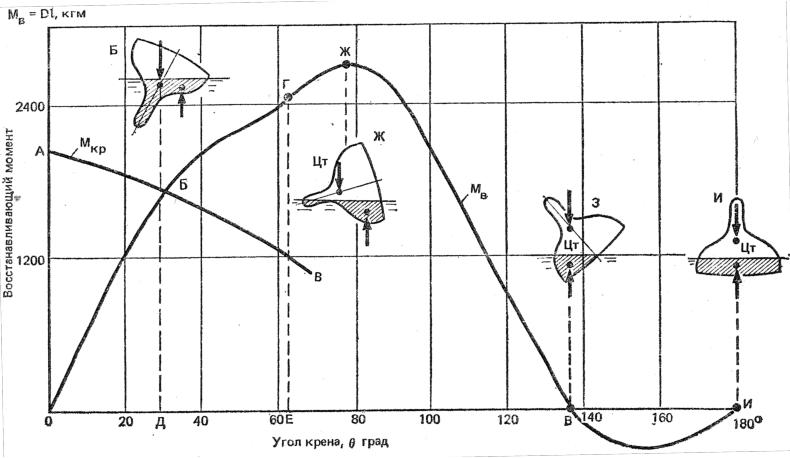
\includegraphics[scale=1.3]{0007P.pdf}
  \caption{Диаграмма статической остойчивости крейсерско-гоночной яхты}
  \label{fig:7}
\end{figure*}

\textbf{Диаграмма статической остойчивости}. Очевидно, что полной характеристикой остойчивости яхты может быть кривая изменения восстанавливающего момента \vidx{M}{В} в зависимости от угла крена $\Theta$ или диаграмма статической остойчивости (рис.~\ris{7}). На диаграмме хорошо различимы моменты максимума остойчивости (Ж) и предельного угла крена, при котором судно, будучи предоставлено само себе, опрокидывается (З \--- угол заката диаграммы статической остойчивости).

С помощью диаграммы капитан судна имеет возможность оценивать, например, способность яхты нести ту или, иную парусность при ветре определенной силы. Для этого на диаграмму остойчивости наносят кривые изменения кренящего момента \vidx{M}{КР} в зависимости от угла крена $\Theta$. Точка Б пересечения обеих кривых указывает на угол крена, который получит яхта при статическом, с плавным нарастанием действии ветра. На рис.~\ris{7} яхта получит крен, соответствующий точке Д, \--- около 29\gr. Для судов, имеющих явно выраженные нисходящие ветви диаграммы остойчивости (швертботов, компромиссов и катамаранов), плавание может, быть допущено только при углах крена, не превышающих точки максимума на диаграмме остойчивости. 

На практике экипажам яхт приходится нередко иметь дело с динамическим действием внешних сил, при котором кренящий момент достигает значительной величины в сравнительно короткий промежуток времени. Такое бывает при шквале или ударе волны в наветренную скулу. В этих случаях важна не только величина кренящего момента, но и кинетическая энергия, сообщаемая судну и поглощаемая работой восстанавливающего момента. 

На диаграмме статической остойчивости работа обоих моментов может быть представлена в виде площадей, заключенных между соответствующими кривыми и осями ординат. Условием равновесия яхты при динамическом воздействии внешних сил будет равенство площадей ОАБВЕ (работа \vidx{M}{КР}) и ОБГВЕ (работа \vidx{M}{В}). Учитывая, что площади ОБВЕ общие, можно рассматривать равенство площадей ОАБ и БГВ. На рис.~\ris{7} видно, что в случае динамического действия ветра угол крена (точка Е, около 62\gr) заметно превышает крен от ветра такой же силы при его статическом действии. 

По диаграмме статической остойчивости может быть определен \textbf{предельный динамический кренящий момент}, опрокидывающий швертбот или угрожающий безопасности яхты с открытым кокпитом. Очевидно, что действие восстанавливающего момента может рассматриваться только до угла заливания кокпита или до начальной точки снижения диаграммы статической остойчивости.

Принято считать, что килевые яхты, снабженные тяжелым балластом, практически неопрокидываемы. Однако в уже упоминавшейся Фастнетской гонке 1979\,г. 77 яхт были опрокинуты на угол крена более 90\gr, причем часть из них некоторое время (от 30 сек до 5 мин) оставалась на плаву вверх килем, а несколько яхт встали потом в нормальное положение через другой борт. Наиболее серьезными повреждениями при этом были потери мачт (на 12 яхтах), падение из своих гнезд аккумуляторов, тяжелых камбузных плит и другого оборудования. К нежелательным последствиям привело и попадание воды внутрь корпусов. Случилось это под динамическим воздействием крутой 9--10\-/метровой волны, профиль которой резко ломался при переходе из океана в мелководное Ирландское море, при ветре скоростью 25\otdo 30\,м/с.

\textbf{Факторы, влияющие на поперечную остойчивость}. Таким образом, мы можем сделать определенные выводы о влиянии различных элементов проекта яхты на её остойчивость. На малых углах крена главную роль в создании восстанавливающего момента играют ширина яхты и коэффициент полноты площади ватерлинии. Чем шире яхта и полнее её ватерлиния, тем дальше от \textit{ДП} смещается \textit{ЦВ} при крене судна, тем больше плечо остойчивости формы. Диаграмма статической остойчивости достаточно широкой яхты имеет более крутую восходящую ветвь, чем узкой, \--- до $\Theta = 60 \motdo 80gr$. 

Чем ниже расположен центр тяжести яхты, тем она остойчивее, причем влияние глубокой осадки и большого балласта сказывается практически по всей диаграмме остойчивости яхты. Занимаясь модернизацией яхты, полезно помнить простое правило: каждый килограмм под ватерлинией повышает остойчивость, а каждый килограмм над ватерлинией ухудшает её. Особенно ощутим для остойчивости тяжелый рангоут и такелаж.

При одинаковом расположении центра тяжести яхта с избыточным надводным бортом имеет и более высокую остойчивость на углах крена более 30\otdo 35\gr, когда на судне с нормальной высотой борта палуба начинает входить в воду. Высокобортная яхта имеет большую величину максимального восстанавливающего момента. Это качество присуще также яхтам, имеющим водонепроницаемые рубки достаточно большого объема. 

Особо следует остановиться на влиянии воды в трюме и жидкостей в цистернах. Дело не только в перемещении масс жидкостей в сторону накрененного борта; главную роль играет наличие свободной поверхности переливающейся жидкости, а именно \--- её момент инерции относительно продольной оси. Если, например, поверхность воды в трюме имеет длину $l$, а ширину $b$, то метацентрическая высота уменьшается на величину

\begin{equation}
  \Delta h = \frac{l \cdot b^3}{\ 12D\ }, \quad \text{м.}
\end{equation}

Особенно опасна вода в трюме, свободная поверхность которого имеет большую ширину. Поэтому при плавании в штормовых условиях воду из трюма нужно своевременно удалять.

Для уменьшения влияния свободной поверхности жидкостей в цистернах устанавливают продольные отбойные переборки, которые по ширине делят на несколько частей. В переборках делают отверстия для свободного перетекания жидкости.

\textbf{Поперечная остойчивость и ходкость яхты.} При увеличении крена сверх 10\otdo 12\gr сопротивление воды движению яхты заметно возрастает, что приводит к потере скорости. Поэтому важно, чтобы при усилении ветра яхта дольше могла нести эффективную парусность, не имея чрезмерного крена.Нередко даже на сравнительно крупных яхтах во время гонок экипаж располагается на наветренном борту, пытаясь уменьшить крен. 

Насколько эффективно перемещение груза (экипажа) на один борт, нетрудно представить по простейшей формуле, которая справедлива для небольших углов (в пределах 0\otdo 10\gr) крена:

\begin{equation}
  \vidx{M}{О} = \frac{D \cdot h}{57,3} \quad ,
\end{equation}

где: \vidx{M}{O} \--- момент, кренящий яхту на 1\gr; $D$ \--- водоизмещение яхты, т; $h$ \--- начальная поперечная метацентрическая высота, м. 

Зная массу перемещаемого груза и расстояние нового места расположения
его от \textit{ДП}, можно определить кренящий момент, а разделив его
на \vidx{M}{О}, получить угол крена в градусах. Например, если на яхте
водоизмещением 7\,т при $h=1\,\text{м}$ пять человек расположатся у
борта на расстоянии 1,5\,м от \textit{ДП}, то создаваемый ими кренящий
момент придаст яхте крен в 4,5\gr (или уменьшит примерно на столько же
крен на другой борт).

\textit{Продольная остойчивость.}\index{остойчивость!продольная} Физика явлений, происходящих при продольных наклонах яхты аналогична явлениям при крене, но продольная метацентрическая высота по величине сравнима с длиной яхты. Поэтому продольные наклоны, дифферент, обычно невелики и измеряются не в градусах, а по изменениям осадки носом и кормой. И, тем не менее, если из яхты выжимают все её возможности, нельзя не считаться с действием сил, дифферентующих яхту на нос и перемещающих центр величины, вперед (см. рис.~\ris{4}). Этому можно противодействовать, перемещая экипаж в кормовую часть палубы. 

Наибольшей величины дифферентующие на нос силы достигают при плавании в бакштаг; на этом курсе, особенно в сильный ветер, экипаж следует смещать, возможно, дальше в корму. На курсе бейдевинд дифферентующий момент невелик, и экипажу лучше всего располагаться близ миделя, откренивая судно. На фордевинде дифферентующий момент оказывается меньше, чем на бакштаге, особенно если яхта несет спинакер и блупер, дающие определенную подъемную силу.

У катамаранов величина продольной метацентрической высоты сравнима с поперечной, иногда меньше нее. Поэтому действие дифферентующего момента, практически незаметное на килевой яхте, может опрокинуть катамаран, таких же главных размерений. Статистика аварий отмечает случаи опрокидывания через нос на попутных курсах крейсерских катамаранов с высокой парусностью. 

\section{Сопротивление дрейфу}

Поперечная сила \vidx{F}{Д} (см. рис.~\ris{4}) не только кренит яхту, она вызывает боковой снос \--- \textbf{дрейф под ветер}. Сила дрейфа зависит от курса яхты относительно ветра. При плавании в крутой бейдевинд она втрое превышает силу тяги, движущую яхту вперед; на галфвинде обе силы примерно равны; в крутой бакштаг (истинный ветер около 135\gr относительно курса яхты) движущая сила оказывается в 2--3 раза больше силы дрейфа, а на чистом фордевинде сила дрейфа вовсе отсутствует. Следовательно, для того чтобы судно успешно продвигалось вперед курсом от бейдевинда до галфвинда, оно должно обладать достаточным боковым сопротивлением дрейфу, намного превышающим сопротивление воды движению яхты по курсу. 

Функцию создания силы сопротивления дрейфу у современных яхт выполняют в основном шверты, плавниковые кили и рули. 

Как мы уже говорили, непременным условием возникновения силы сопротивления дрейфу является движение яхты под небольшим углом к \textit{ДП} \--- углом дрейфа. Рассмотрим, что при этом происходит в потоке воды непосредственно у киля, который представляет собой крыло с поперечным сечением в виде тонкого симметричного аэродинамического профиля (рис.~\ris{8}).

\begin{figure*}[htb]
  \centering
  \includegraphics[scale=1.3]{0008P.pdf}
  \caption{Образование подъемной силы на крыле}
  \label{fig:8}
  \centering{}\small \textit{a} \--- обтекание профиля при $\alpha = 0$;
                     \textit{б}~и~\textit{в} \--- образование стартового вихря;
                     \textit{г} \--- отрыв стартового вихря;
                     \textit{д} \--- появление устойчивой циркуляции потока вокруг крыла;
                     \textit{е} \--- схема действующих сил при развитой циркуляции
\end{figure*}

Если угол дрейфа отсутствует (рис.~\ris{8},~\textit{а}), то поток воды, встречаясь с профилем киля в точке \textit{а}, разделяется на две части. В этой точке, называемой критической, скорость потока равна 0, давление максимальное, равное скоростному напору $(\rho \cdot v^2) / 2$, где: $\rho$ \--- массовая плотность воды (для пресной воды = 102 $\text{кгс}^2 / \text{м}^4$ ); $v$ \--- скорость движения яхты (м/с). 

И верхняя и нижняя части потока одновременно обтекают поверхности профиля и вновь встречаются в точке \textit{b} на выходящей кромке. Очевидно, что никакой силы, направленной поперек потока, на профиле возникнуть не может; будет действовать только одна сила сопротивления трения, обусловленная вязкостью воды. 

Если же профиль отклонить на некоторый угол атаки $\alpha$ (в случае яхтенного киля \--- угол дрейфа), то картина обтекания профиля изменится (рис.~\ris{8},~\textit{б}). Критическая точка $a$ переместится на нижнюю часть <<носика>> профиля. Путь, который должна пройти частица воды вдоль верхней поверхности профиля, удлинится, а точка $b_1$, где по условиям неразрывности потока должны были бы встретиться частицы, обтекающие верхнюю и нижнюю поверхности профиля, пройдя равный путь, оказывается на верхней поверхности. Однако при огибании острой выходящей кромки профиля нижняя часть потока срывается с кромки в виде вихря (рис.~\ris{8},~\textit{в} и \textit{г}). Этот вихрь, называемый стартовым, вращаясь против часовой стрелки, вызывает циркуляцию воды вокруг профиля в обратном направлении, т.\=,е. по часовой стрелке (рис.~\ris{8},~\textit{д}). Данное явление, вызванное силами вязкости, аналогично вращению большого зубчатого колеса (циркуляция), находящегося в зацеплении с малой ведущей шестерней (стартовый вихрь). 

После того как возникает циркуляция, стартовый вихрь срывается с выходящей кромки, точка $b_2$ перемещается ближе к этой кромке, вследствие чего здесь больше не существует разности скоростей, с которыми крыло покидают верхняя и нижняя части потока. Циркуляция же вокруг крыла становится причиной возникновения подъемной силы \ve Y, направленной поперек потока: у верхней поверхности крыла скорость частиц воды за счет циркуляции увеличивается, у нижней, встречаясь с частицами, вовлеченными в циркуляцию, \--- затормаживается. Соответственно у верхней поверхности давление понижается по сравнению с давлением в потоке перед крылом, а у нижней поверхности \--- повышается. Разность давлений и дает подъемную силу \ve Y. 

Кроме того, на профиль будет действовать \textbf{сила лобового (профильного) сопротивления} \ve X, возникающая вследствие трения воды о поверхность профиля и гидродинамического давления на его переднюю часть.

\begin{figure}[htb]
  \centering
  \includegraphics[scale=1.2]{0009P.pdf}
  \caption{Распределение давления по ширине симметричного аэродинамического профиля при угле атаки $\alpha = 7\gr$}
  \label{fig:9}
\end{figure}

На рис.~\ris{9} представлены результаты замера давления у поверхности симметричного профиля, сделанного в аэродинамической трубе. По оси ординат отложено значение коэффициента $C_P$, который представляет собой отношение избыточного давления (полное давление минус атмосферное) к скоростному напору $(\rho \cdot v^2) / 2$. На верхней стороне профиля давление отрицательное (разрежение), на нижней \--- положительное. Таким образом, подъемная сила, действующая на любой элемент профиля, складывается из действующих на него сил давления и разрежения, а в целом она пропорциональна площади, заключенной между кривыми распределения давления по хорде профиля (на рис.~\ris{9} заштриховано).

Данные, представленные на рис.~\ris{9}, позволяют сделать ряд важных выводов о работе яхтенного киля. Во-первых, главную роль в создании боковой силы играет разрежение, возникающее на поверхности плавника со стороны наветренного борта. Во-вторых, пик разрежения располагается вблизи входящей кромки киля. Соответственно точка приложения результирующей подъемной силы находится на передней трети хорды плавника. В целом же подъемная сила возрастает вплоть до угла атаки 15\otdo 18\gr, после чего внезапно падает.

Вследствие образования завихрения на стороне разрежения плавное обтекание крыла нарушается, разрежение падает и происходит срыв потока (это явление более подробно рассмотрено в гл.~\ref{chap:2} для парусов). Одновременно с увеличением угла атаки возрастает лобовое сопротивление \--- оно достигает максимума при $\alpha = 90\gr$.

Величина дрейфа современной яхты редко превышает 5\gr, так что срыв, потока с киля можно не опасаться. Однако критический угол атаки должен учитываться для яхтенных рулей, которые проектируются и работают также по принципу крыла. 

Рассмотрим основные параметры яхтенных килей, которые оказывают существенное влияние на их эффективность в создании силы сопротивлению дрейфу. В равной степени изложенное далее можно распространить и на рули с учетом того, что они работают со значительно большим углом атаки.

\textbf{Толщина и форма поперечного сечения киля.} Испытания симметричных аэродинамических профилей показали, что более толстые профили (с большей величиной отношения толщины сечения $t$ к его хорде $b$) дают большую подъемную силу. Их лобовое сопротивление выше, чем у профилей с меньшей относительной толщиной. Оптимальные результаты могут быть получены при $t/b = 0,09 \motdo 0,12$. Величина подъемной силы на таких профилях сравнительно мало зависит от скорости яхты, поэтому кили развивают достаточную силу сопротивления дрейфа и в слабый ветер. 

Существенное влияние на величину силы сопротивления дрейфу оказывает положение максимальной толщины профиля по длине хорды. Наиболее эффективными оказываются профили, у которых максимальная толщина расположена на расстоянии 40\otdo 50\,\% хорды от их <<носика>>. Для яхтенных рулей, работающих под большими углами атаки, используют профили с максимальной толщиной, расположенной несколько ближе к передней кромке, \--- до 30\,\% хорды.

Определенное влияние на эффективность киля оказывает форма, <<носика>> профиля \--- радиус округления входящей кромки. Если кромка слишком острая, то набегающий на киль поток получает здесь большое ускорение и срывается с профиля в виде вихрей. При этом происходит падение подъемной силы, особенно существенное при больших углах атаки. Поэтому подобное заострение входящей кромки недопустимо для рулей. 

\textbf{Аэродинамическое удлинение.} У концов крыла обнаруживается перетекание воды из области повышенного давления на спинку профиля. В результате с концов крыла срываются вихри, образующие две вихревые дорожки. На их поддержание затрачивается довольно значительная часть энергии, образуя так называемое \textbf{индуктивное сопротивление}. Кроме того, вследствие выравнивания давлений у концов крыла происходит местное падение подъемной силы, как это показано на эпюре распределения её по длине крыла на рис.~\ris{10}. 

\begin{figure*}[htb]
  \centering
  \includegraphics[scale=1.3]{0010P.pdf}
  \caption{Схема обтекания крыла конечного размаха}
  \label{fig:10}
  \centering
  \small
  \textit{1} \--- распределение подъемной силы по длине крыла;
  \textit{2} \--- циркуляция;
  \textit{3} \--- перетекание жидкости по концам крыла;
  \textit{4} \--- концевые вихри;
  \textit{5} \--- распределение вызванных скоросте по размаху крыла $L$
\end{figure*}

Чем короче длина крыла $L$ по отношению к его хорде $b$, т.\=,е. чем меньше его удлинение $L/b$, тем относительно больше потеря подъемной силы и тем больше индуктивное сопротивление. В аэродинамике принято оценивать удлинение крыла по формуле $\lambda = L^2/S$ (где $S$ \--- площадь крыла), которая может быть применена для крыльев и плавников любых очертаний. При прямоугольной форме аэродинамическое удлинение равно соотношению $\lambda = L / b$; для треугольного крыла $\lambda = 2 \cdot L / b$.
На рис.~\ris{10} показано крыло, составленное из двух трапециевидных плавниковых килей. На яхте киль крепится широким основанием к днищу, поэтому здесь перетекание воды на сторону разрежения отсутствует и под влиянием корпуса давления на обоих поверхностях выравнивается. Без этого влияния можно было бы считать аэродинамическое удлинение вдвое большим, чем отношение глубины киля к его осадке. На практике же это отношение, зависящее от размеров киля, обводов яхты и угла крена превышается только в 1,2\otdo 1,3 раза.

\begin{figure}[htb]
  \centering
  \includegraphics[scale=1.2]{0011P.pdf}
  \caption{Зависимость сопротивления дрейфу от удлинения киля и угла атаки}
  \label{fig:11}
\end{figure}

Влияние аэродинамического удлинения киля на величину развиваемой им силы сопротивления дрейфу \vidx{R}{Д} можно оценить по результатам испытаний плавника, имеющего профиль NACA 009 ($t/b = 9\,\%$) и площадь 0,37\msq (рис.~\ris{11}). Скорость потока соответствовала скорости движения яхты 3 узла (1,5\,м/с). Интерес представляет изменение силы сопротивления дрейфу при угле атаки 4\otdo 6\gr, что соответствует углу дрейфа яхты на курсе бейдевинд. Если принять силу \vidx{R}{Д} при удлинении $\lambda = 1$ за единицу (6,8 при $\alpha = 5\gr$), то при увеличении $\lambda$ до 2 сопротивление дрейфу увеличивается более чем в 1,5 раза (10,4\,кг), а при $\lambda = 3$ \--- ровно вдвое (13,6\,кг). Этот же график может служить для качественной оценки эффективности рулей различного удлинения, которые работают в области больших углов атаки.

Таким образом, увеличивая удлинение плавника киля, можно получить необходимую величину боковой силы \vidx{R}{Д} при меньшей площади киля и, следовательно, при меньшей площади смоченной поверхности и сопротивлении воды движению яхты. Удлинение килей на современных крейсерско\-/гоночных яхтах составляет в среднем $\lambda = 1 \motdo 3$. Перо руля, служащее не только для управления судном, но и являющееся составным элементом в создании сопротивления яхты, имеет еще большее удлинение, приближающееся к $\lambda = 4$. 

\textbf{Площадь и формы киля.} Чаще всего размеры киля определяют по статистическим данным, сравнивая проектируемую яхту с хорошо зарекомендовавшими себя судами. На современных крейсерско\-/гоночных яхтах с раздельным от киля рулем суммарная площадь киля и руля составляет от 4,5 до 6,5\,\% площади парусности яхты, а площадь руля \--- 20\otdo 40\,\% площади киля.

Для получения оптимального удлинения конструктор яхты стремится принять осадку наибольшей допускаемой по условиям плавания или правилами обмера. Чаще всего киль имеет вид трапеции с наклонной передней кромкой. Как показали исследования, для яхтенных килей, имеющих удлинение от 1 до 3, угол между передней кромкой и вертикалью в пределах от -8\gr до 22,5\gr практически не влияет на гидродинамические характеристики киля. Если киль (или шверт) очень узкий и длинный, то наклон передней кромки более 15\gr к вертикали сопровождается отклонением линий тока воды вниз по профилю \--- по направлению к нижнему заднему углу. Вследствие этого падает подъемная сила и возрастает лобовое сопротивление киля. В данном случае оптимальный угол наклона составляет 5\gr к вертикали. 

На величину подъемной силы, развиваемой килем и рулем, значительно влияет качество отделки его поверхности, особенно передней кромки, где формируется поток, обтекающий профиль. Поэтому рекомендуется полировать киль и руль на расстоянии не менее 1,5\,\% хорды профиля.

\textbf{Скорость яхты.} Подъемная сила на любом крыле определяется по формуле:

\begin{equation}
  \ve Y = C_Y \cdot \frac{\rho \cdot v^2}{2} \cdot S, \text{кгс,} 
\end{equation}

где: $C_Y$ \--- коэффициент подъемной силы, зависящий от параметров крыла \--- формы профиля, удлинения, очертаний в плане, а также от угла атаки \--- с увеличением угла атаки он возрастает; $\rho$ \--- массовая плотность воды, кгс$^2$/м$^4$; $v$ \--- скорость потока, обтекающего крыло, м/с; $S$ \--- площадь крыла,\msq.
 
Таким образом, сила сопротивления дрейфу \--- величина переменная, пропорциональная квадрату скорости. В начальный момент движения яхты, например, после поворота оверштаг, когда судно теряет ход, или при отходе от бона в прижимной ветер, подъемная сила на киле невелика. Для того чтобы сила \ve Y сравнялась с силой дрейфа \vidx{F}{Д}, киль должен расположиться к набегающему потоку под большим углом атаки. Иными словами, судно начинает движение с большим углом дрейфа. По мере набора скорости угол дрейфа уменьшается, пока не достигнет своей нормальной величины \--- 3\otdo 5\gr.

Это обстоятельство должен учитывать капитан, предусматривая достаточно места с подветра при разгоне яхты или после поворота на новый галс. Большой начальный угол дрейфа необходимо использовать для скорейшего набора скорости, слегка потравив шкоты. Кстати, благодаря этому уменьшается сила дрейфа на парусах. 

Необходимо также помнить механику возникновения подъемной силы, которая появляется на киле только после отрыва стартового вихря и развития устойчивой циркуляции. На узком киле современной яхты циркуляция возникает быстрее, чем на корпусе яхты с навесным на киле рулем, т.\=,е. на крыле с большой хордой. Вторая яхта больше сдрейфует под ветер, прежде чем корпус начнет эффективно препятствовать дрейфу.

\section{Управляемость}

Управляемостью называется качество судна, позволяющее ему следовать по заданному курсу или изменять направление движения. Управляемой может считаться только та яхта, которая реагирует нужным образом на перекладку руля.

Управляемость объединяет два свойства судна \--- устойчивость на курсе и поворотливость.

\textbf{Устойчивость на курсе} \--- это способность яхты удерживать заданное прямолинейное направление движения при действии на нее различных внешних сил: ветра, волнения и т.\=,п. Устойчивость на курсе зависит не только от конструктивных особенностей яхты и характера действия внешних сил, но и от реакции рулевого на отклонение судна от курса, его чутья руля.

Обратимся вновь к схеме действия внешних сил на паруса и корпус яхты (см. рис.~\ris{4}). Решающее значение для устойчивости яхты на курсе имеет взаимное расположение двух пар сил. Кренящая сила \vidx{F}{Д} и сила сопротивления дрейфу \vidx{R}{Д} стремятся увалить нос яхты под ветер, в то время как вторая пара \--- сила тяги \ve T и сопротивление движению \ve R приводит яхту к ветру. Очевидно, что реакция яхты зависит от соотношения величины рассматриваемых сил и плеч $a$ и $b$, на которых они действуют. При увеличении угла крена плечо приводящей пары $b$ также увеличивается. Плечо уваливающей пары, $a$ зависит от взаимного расположения центра парусности (\textit{ЦП}) \--- точки приложения результирующей аэродинамических сил к парусам и центра бокового сопротивления (\textit{ЦБС}) \--- точки приложения результирующей гидродинамических сил к корпусу яхты. Положение этих точек изменяется в зависимости от многих факторов: курса яхты относительно ветра, формы и настройки парусов, крена и дифферента яхты, формы и профиля киля и руля и т.\=,п.

\begin{figure}[htb]
  \centering
  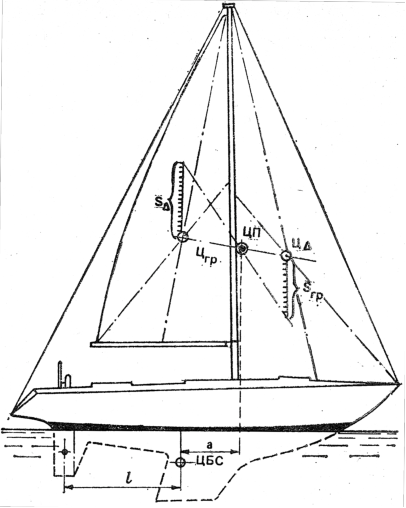
\includegraphics[scale=1.2]{0012P.pdf}
  \caption{Схема определения геометрического центра парусности яхты с вооружением типа <<шлюп>>}
  \label{fig:12}
\end{figure}

Поэтому при проектировании и перевооружении яхт оперируют с условными \textit{ЦП} и \textit{ЦБС}, считая их расположенными в центрах тяжести плоских фигур, которыми являются паруса, поставленные в диаметральной плоскости яхты, и подводные очертания \textit{ДП} с килем, плавниками и рулем (рис.~\ris{12}). 

Известно, что центр тяжести треугольного паруса располагается на пересечении двух медиан, а общий центр тяжести двух парусов находится на отрезке прямой, соединяющей \textit{ЦП} обоих парусов, и делит этот отрезок обратно пропорционально их площади. Обычно, в расчет принимается не фактическая площадь стакселя, а обмерная площадь переднего парусного треугольника. 

Положение \textit{ЦБС} можно определить, уравновешивая на острие иголки профиль подводной части \textit{ДП}, вырезанный из тонкого картона. Когда шаблон располагается строго горизонтально, игла находится в условной точке \textit{ЦБС}. Напомним, что в создании силы сопротивления дрейфу главная роль принадлежит плавниковому килю и рулю. Центры гидродинамических давлений на их профилях могут быть найдены достаточно точно, например, для профилей с относительной толщиной $t/b$ около 8\,\% эта точка находится на расстоянии около 26\,\% хорды от входящей кромки. Однако корпус яхты, хотя и участвует в создании поперечной силы в малой степени, вносит определенные изменения в характер обтекания киля и руля, причем он изменяется в зависимости от угла крена и дифферента, а также скорости яхты. В большинстве случаев на курсе бейдевинд истинный \textit{ЦБС} перемещается вперед. 

Конструкторы, как правило, располагают \textit{ЦП} на некотором расстоянии (опережении) впереди \textit{ЦБС}. Обычно опережение задается в процентах длины судна по ватерлинии и составляет для бермудского шлюпа 15\otdo 18\,\% \lkvl.

Если истинный \textit{ЦП} оказывается расположенным слишком далеко впереди \textit{ЦБС}, яхта на курсе бейдевинд уваливается под ветер и рулевому приходится постоянно держать руль отклоненным на ветер. Если же \textit{ЦП} оказывается позади \textit{ЦБС}, то яхта стремится привестись к ветру; требуется постоянная работа рулем, чтобы сдерживать судно. 

Особенно неприятна тенденция яхты к уваливанию. В случае аварии с рулем яхту не удается с помощью одних парусов привести на курс бейдевинд, кроме того, она обладает повышенным дрейфом. Дело в том, что киль яхты отклоняет стекающий с него поток воды ближе к \textit{ДП} судна. Поэтому если руль стоит прямо, он работает с заметно меньшим углом атаки, чем киль. Если отклонить руль в наветренную сторону, то образуемая на нем подъемная сила оказывается направленной в подветренную сторону \--- туда же, что и сила дрейфа на парусах. В данном случае киль и руль <<тянут>> в разные стороны и яхта неустойчива на курсе.

Иное дело легкая тенденция яхты приводиться. Переложенный на небольшой угол (3\otdo 4\gr) под ветер руль работает с таким же или несколько большим углом атаки, что и киль, и эффективно участвует в сопротивлении дрейфу. Поперечная сила, возникающая на руле, вызывает значительное смещение общего \textit{ЦБС} к корме, одновременно уменьшается угол дрейфа, яхта устойчиво лежит на курсе.

Однако если на курсе бейдевинд руль приходится постоянно перекладывать под ветер на большую величину, чем 3\otdo 4\gr, следует подумать о корректировке относительного положения \textit{ЦБС} и \textit{ЦП}. На уже построенной яхте это проще делать, перемещая вперед \textit{ЦП}, \--- устанавливая мачту в степсе в крайнее носовое положение или наклоняя её вперед. Причиной приведения яхты может быть также грот \--- слишком <<пузатый>> или с перебранной задней шкаториной. В этом случае полезен промежуточный штаг, с помощью которого можно придать мачте в средней части (по высоте) прогиб вперед и тем самым сделать парус более плоским, а также ослабить заднюю шкаторину. Можно также укоротить длину нижней шкаторины грота. 

Сложнее сместить в корму \textit{ЦБС}, для чего нужно установить кормовой плавничок перед рулем или увеличить площадь пера руля.

Мы уже говорили, что при увеличении крена увеличивается, и тенденция яхты приводиться. Это происходит не только вследствие увеличения плеча приводящей пары сил \--- \ve T и \ve R. При крене гидродинамическое давление в районе носовой волны повышается, что приводит к смещению \textit{ЦБС} вперед. Поэтому в свежий ветер для уменьшения тенденции яхты приводиться следует переместить вперед и \textit{ЦП}: взять риф на гроте или немного перетравить его для данного курса. Полезно также сменить стаксель на меньший по площади, благодаря чему уменьшается крен и дифферент яхты на нос.

Опытный конструктор при выборе величины опережения а обычно учитывает остойчивость яхты, чтобы компенсировать рост приводящего момента при крене: для яхты с меньшей остойчивостью задается большая величина опережения, для более остойчивых судов опережение принимается минимальным.

Хорошо уцентрованные яхты часто обладают повышенной рыскливостью на курсе бакштаг, когда потравленный на борт грот стремится развернуть яхту носом к ветру. Этому помогает и высокая волна, набегающая с кормы под углом к ДП. Чтобы одерживать яхту на курсе, приходится сильно работать рулем, отклоняя его на критический угол, когда возможен срыв потока с его подветренной поверхности (обычно это случается при углах атаки a 15\otdo 20\gr). Это явление сопровождается потерей подъемной силы на руле и, следовательно, управляемости яхты. Яхта внезапно может резко броситься к ветру и получить большой крен, при этом из-за уменьшения углубления пера руля на сторону разрежения может прорваться воздух с поверхности воды. 

Борьба с этим явлением, получившим название \textbf{брочинг}, заставляет увеличивать площадь пера руля и его удлинение, устанавливать перед рулем плавник, площадь которого составляет около четверти площади пера. Благодаря наличию плавника перед рулем организуется направленный поток воды, увеличиваются критические углы атаки руля, предотвращается прорыв воздуха к нему и уменьшается усилие на румпеле. При плавании в бакштаг экипаж должен стремиться к том чтобы тяга спинакера была направлена по возможности вперед, а не вбок чтобы избежать излишнего крена. Важно также препятствовать появлению дифферента на нос, при котором может уменьшиться углубление руля. Брочингу способствует также бортовая качка яхты, появляющаяся вследствие срывов потока воздуха со спинакера.

Устойчивость на курсе помимо рассмотренного влияния внешних сил и взаимного расположения их точек приложения определяется конфигурацией подводной части \textit{ДП}. Ранее для дальних плаваний по открытой воде отдавали предпочтение яхтам с длинной килевой линией, как обладающим большим сопротивлением повороту и соответственно \--- устойчивостью на курсе. Однако этому типу судов свойственны существенные недостатка например большая смоченная поверхность и плохая поворотливость. К тому же выяснилось, что устойчивость на курсе зависит не столько от величины боковой проекции \textit{ДП}, сколько от положения руля относительно \textit{ЦБС}, т.\=,е. от <<рычага>>, на котором действует руль. Отмечено, что если это расстояние оказывается менее 25\,\% \lkvl, то яхта становится рыскливой и плохо реагирует на отклонение руля. При $l = 40 \motdo 45\,\%$ \lkvl (см. рис.~\ris{12}) удержание судна на заданном курсе не составляет труда.

\begin{figure*}[htb]
  \centering
  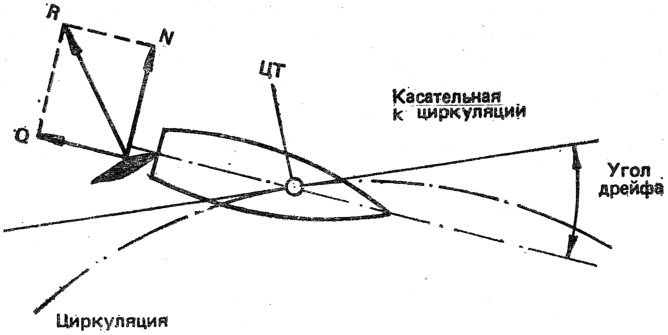
\includegraphics{0013P.pdf}
  \caption{Действие руля и схема движения яхты на циркуляции}
  \label{fig:13}
\end{figure*}

\textbf{Поворотливость} \--- способность судна изменять направление движения, описывать траекторию под действием руля и парусов. Действие руля основано на том же принципе гидродинамического крыла, что рассматривался и для яхтенного киля. При перекладке руля на некоторый угол возникает гидродинамическая сила \ve R, одна из составляющих которой \ve N толкает корму яхты в сторону, противоположную той, в которую положен руль (рис.~\ris{13}). Под её действием судно начинает двигаться по кривой траектории. Одновременно сила \ve R дает составляющую \ve Q \--- силу сопротивления, тормозящую ход яхты.

Если закрепить руль в одном положении, то судно пойдет примерно по окружности, называемой циркуляцией. Диаметр или радиус циркуляции является мерой поворотливости судна: чем больше радиус циркуляции, тем хуже поворотливость. По циркуляции движется только центр тяжести яхты, корму выносит наружу. Одновременно судно получает дрейф, вызванный центробежной силой и отчасти силой \ve N на пере руля.

Радиус циркуляции зависит от скорости и массы яхты, её момента инерции относительно вертикальной оси, проходящей через \textit{ЦТ}, от эффективности руля \--- величины силы \ve N и её плеча относительно \textit{ЦТ} при данном отклонении руля. Чем больше скорость и водоизмещение яхты, чем больше тяжелых масс (двигатель, якоря, детали оборудования) размещено в оконечностях судна, тем больше радиус циркуляции. Обычно радиус циркуляции, определенный на ходовых испытаниях яхты, выражают в длинах корпуса.

Поворотливость тем лучше, чем короче подводная часть судна и чем ближе к миделю сконцентрирована её основная площадь. Плохой поворотливостью обладают, например, суда с длинной килевой линией (типа военно\-/морских шлюпок) и, наоборот, хорошей \--- швертботы с узкими глубокими швертами. 

Эффективность руля зависит от площади и формы пера, профиля поперечного сечения, аэродинамического удлинения, типа установки (на ахтерштевне, отдельно от киля или на плавнике), а также расстояния баллера от \textit{ЦБС}. Наибольшее распространение получили рули, спроектированные в виде крыла с аэродинамическим профилем поперечного сечения. Максимальной толщина профиля принимается обычно в пределах 10\otdo 12\,\% хорды и располагается на 1/3 хорды от передней кромки. Площадь руля составляет обычно 9,5\otdo 11\,\% площади погруженной части \textit{ДП} яхты. 

Руль с большим удлинением (отношение квадрата глубины погружения руля к его площади) развивает большую поперечную силу на малых углах атаки, благодаря чему он эффективно участвует в обеспечении боковой силы сопротивления дрейфу. Однако, как было показано на рис.~\ris{11}, на определенных углах атаки профилей различного удлинения происходит отрыв потока от поверхности разрежения, после чего подъемная сила на профиле существенно падает. Например, при $\lambda = 6$ критический угол перекладки руля составляет 15\gr; при $\lambda = 2$ составляет 30\gr. В качестве компромисса применяют рули с удлинением $\lambda = 4 \motdo 5$ (соотношение сторон прямоугольного руля 2\otdo 2,5), а для повышения критического угла перекладки устанавливают перед рулем плавник\-/скег. Руль с большим удлинением быстрее реагирует на перекладку, так как циркуляция потока, обусловливающая подъемную силу, быстрее развивается вокруг профиля с малой хордой, чем вокруг всей подводной части корпуса с навесным на ахтерштевне рулем. 

Верхняя кромка руля должна плотно прилегать к корпусу в пределах рабочих отклонений $\pm 30\gr$, чтобы препятствовать перетеканию воды через нее; в противном случае эффективность работы руля ухудшается. Иногда на пере руля, если он навешен на транце, закрепляют аэродинамическую шайбу в виде широкой пластины близ ватерлинии.

Сказанное о форме килей применимо и к рулям: оптимальной считается трапециевидная форма с прямоугольной либо слегка скругленной нижней кромкой. Для уменьшения усилий на румпеле руль иногда делают балансирного типа \--- с осью вращения, расположенной на 1/4\otdo 1/5 хорды от <<носика>> профиля.

При управлении яхтой необходимо учитывать специфику работы руля в различных условиях, и, прежде всего срыв потока с его спинки. Нельзя делать резких перекладок руля на борт в начале поворота \--- произойдет срыв потока, поперечная сила \ve N на руле упадет, зато быстро увеличится сила сопротивления \ve R. Яхта будет входить в циркуляцию медленно и с большой потерей скорости. Начинать поворот необходимо, переложив руль на небольшой угол, но как только корма покатится наружу, и угол атаки руля начнет уменьшаться, его следует переложить на больший угол относительно \textit{ДП} яхты. 

Следует помнить, что поперечная, сила на руле быстро возрастает с увеличением скорости яхты. В слабый ветер бесполезно пытаться повернуть яхту быстро, перекладывая руль на большой угол (кстати, величина критического угла зависит от скорости: на меньшей скорости отрыв потока происходит при меньших углах атаки).

Сопротивление руля при изменении курса яхты в зависимости от его формы, конструкции и расположения составляет от 10 до 40\,\% общего сопротивления яхты. Поэтому к технике управления рулем (и к центровке яхты, от которой зависит устойчивость на курсе) надо относиться весьма серьезно, не допускать отклонения руля на больший угол, чем это необходимо.

\section{Ходкость}

\textbf{Ходкостью} называют способность яхты развивать определенную скорость при эффективном использовании энергии ветра.

Скорость, которую может развить яхта, зависит прежде всего от скорости ветра, поскольку все аэродинамические силы, действующие на парус в том числе и сила тяги, возрастав пропорционально квадрату скорости вымпельного ветра. Кроме того, она зависит и от энерговооруженности судна \--- отношения площади парусности к его размерениям. В качестве характеристики энерговооруженности чаще всего применяют отношение $S^{1/2} / V^{1/3}$
(где $S$ \--- площадь парусности\msq; $V$ \--- полное водоизмещение, м$^3$); или $S / \Omega$ 
(здесь $\Omega$ \--- смоченная поверхность корпуса, включая киль и руль). Сила тяги, а, следовательно, и скорость яхты, определяется еще и способностью парусного вооружения развивать достаточную тягу на различных курсах по отношению к направлению ветра.

Перечисленные факторы относятся к парусам \--- движителю яхты, преобразующему энергию ветра в движущую силу \ve T. Как было показано на рис.~\ris{4}, эта сила при равномерном движении яхты должна быть равна и противоположно направлена силе сопротивления движению \ve R. Последняя представляет собой проекцию результирующих всех гидродинамических сил, действующих на смоченную поверхность корпуса, на направление движения.

Различают два рода гидродинамических сил: силы давления, направленные перпендикулярно поверхности корпуса, и силы вязкости, действующие по касательной к этой поверхности. Результирующая сил вязкости дает силу \textbf{сопротивления трения}. 

Силы давления обусловлены образованием при движении яхты волн на поверхности воды, поэтому их результирующая дает силу \textbf{волнового сопротивления}. 

При большой кривизне поверхности корпуса в кормовой части пограничный слой может отрываться от обшивки, могут образовываться завихрения, поглощающие часть энергии движущей силы. Так возникает еще одна составляющая сопротивления движению яхты \--- \textbf{сопротивление формы}.

Еще два вида сопротивления появляются в связи с тем, что яхта движется не прямо вдоль \textit{ДП}, а с некоторым углом дрейфа и с креном. Это \textbf{индуктивное} и \textbf{креновое} сопротивления. Существенную долю в индуктивном сопротивлении занимает сопротивление выступающих частей \--- киля и руля.

Наконец, движению яхты вперед оказывает сопротивление и воздух, омывающий корпус, экипаж, развитую систему тросов такелажа и паруса. Эта часть сопротивления носит название \textbf{воздушного}. 

\textbf{Сопротивление трения.} При движении яхты частицы воды, непосредственно примыкающие к обшивке корпуса, как бы прилипают к ней и увлекаются вместе с судном. Скорость этих частиц относительно корпуса равна нулю (рис.~\ris{14}). Следующий слой частиц, скользя по первому, уже немного отстает от соответствующих точек корпуса, а на определенном расстоянии от обшивки вода вообще остается неподвижной или имеет скорость относительно корпуса, равную скорости яхты $v$. Этот слой воды, в котором действуют силы вязкости, а скорость движения частиц воды относительно корпуса возрастает от 0 до скорости судна, называется пограничным слоем. Толщина его относительно невелика и составляет от 1 до 2\,\% длины корпуса по ватерлинии, однако характер или режим движения частиц воды в нем оказывает существенное влияние на величину сопротивления трения.

\begin{figure*}[htb]
  \centering
  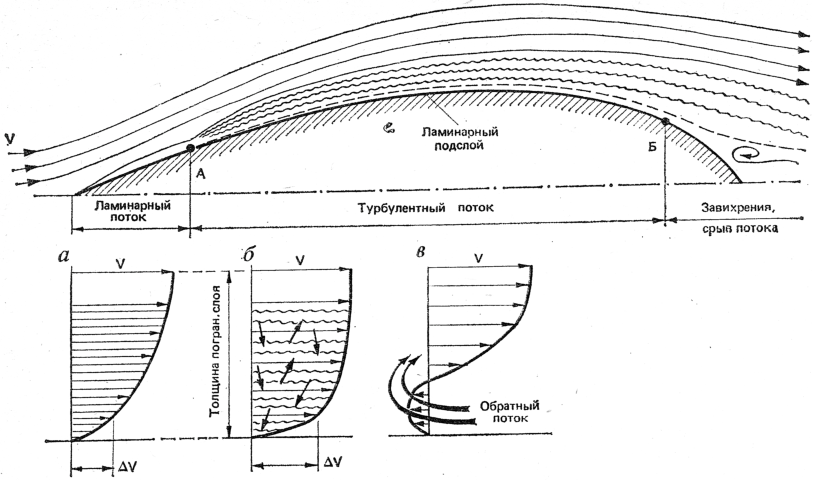
\includegraphics[scale=1.3]{0014P.pdf}
  \caption{Потоки жидкости около корпуса яхты}
  \label{fig:14}
  \small
  \centering{}
  \textit{А} \--- точка перехода ламинарного пограничного слоя в турбулентный; \textit{Б} \--- точка отрыва потока от корпуса; \textit{а} \--- изменение скоростей потока в ламинарном пограничном слое; \textit{б} \--- изменение скоростей потока в турбулентном слое; \textit{в} \--- изменение скоростей в пограничном слое в корму от точки \textit{Б}
\end{figure*}

Установлено, что режим движения частиц изменяется в зависимости от скорости судна и длины его смоченной поверхности. В гидродинамике эта зависимость выражается числом Рейнольдса:

\begin{equation}
  \Renum = \frac{v \cdot L}{\nu} \quad , 
\end{equation}

где: $\nu$ \--- коэффициент кинематической вязкости воды (для пресной воды $\nu = 1,15 \cdot 10^{-6} \text{м}^2/\text{с})$; $L$ \--- длина смоченной поверхности, м; $v$ \--- скорость яхты, м/с. 

При относительно небольшом числе $\Renum = 10^6$ частицы воды в пограничном слое движутся слоями, образуя ламинарный поток. Его энергии оказывается недостаточно, чтобы преодолеть силы вязкости, препятствующие поперечным перемещениям частиц. Наибольший перепад скорости между слоями частиц оказывается непосредственно у поверхности корпуса; соответственно и силы трения имеют здесь наибольшую величину. 

Число Рейнольдса в пограничном слое увеличивается по мере удаления частиц воды от форштевня (с возрастанием смоченной длины). При скорости 2 м/с, например, уже на расстоянии около 2 м от него Re достигнет критической величины, при которой режим потока в пограничном слое становится вихревым, т.\=,е. турбулентным и направленным поперек пограничного слоя. Вследствие возникшего обмена кинетической энергией между слоями скорость частиц близ поверхности корпуса растет в большей степени, чем при ламинарном потоке. Перепад скоростей $\Delta v$ здесь возрастает, соответственно растет и сопротивление трения. Вследствие поперечных движений частиц воды толщина пограничного слоя увеличивается, а сопротивление трения резко увеличивается. 

Ламинарный режим обтекания охватывает только небольшую часть корпуса яхты в носовой его части только на малых скоростях. Критическая величина Re, при которой возникает турбулентное обтекание корпуса, лежит в пределах $5 \cdot 10^5\motdo 6 \cdot 10^6$ и в значительной степени зависит от формы и гладкости поверхности его. При повышении скорости точка перехода, ламинарного пограничного слоя в турбулентный перемещается в сторону носа. При достаточно высокой скорости может наступить момент, когда вся смоченная поверхность корпуса будет охвачена турбулентным потоком. Правда, непосредственно около обшивки, где скорость обтекания близка к нулю, все же сохраняется тончайшая пленка с ламинарным режимом \--- ламинарный подслой. 

Сопротивление трения рассчитывают по формуле:

\begin{equation}
  \cidx{R}{ТР} = \cidx{\zeta}{ТР} \cdot \frac{\rho \cdot v^2}{2} \cdot \Omega, \quad \text{кгс}, 
\end{equation}

где: \cidx{R}{ТР} \--- сопротивление трения, кг; \cidx{\zeta}{ТР} \--- коэффициент сопротивления трения; $\rho$ \--- массовая плотность воды; для пресной воды: $\rho = 102\, \text{кг} \cdot \text{с}^2/\text{м}^4$; $v$ \--- скорость яхты, м/с; $\Omega$ \--- смоченная поверхность,\msq. 

Коэффициент сопротивления трения \--- величина переменная, зависящая от характера потока в пограничном слое, длины корпуса \lkvl, скорости $v$ и шероховатости поверхности корпуса.

На рис.~\ris{15} показaнa зависимость коэффициента сопротивления трения \cidx{\zeta}{ТР} от числа Re и шероховатости поверхности корпуса.

\begin{figure*}[htb]
  \centering
  \includegraphics[scale=1.3]{0015P.pdf}
  \caption{Коэффициент сопротивления трения технически гладкой и шероховатых поверхностей в зависимости от числа Рейнольдса \Renum}
  \label{fig:15}
\end{figure*}

Рост сопротивления шероховатой поверхности по сравнению с гладкой нетрудно объяснить наличием в турбулентном пограничном слое ламинарного подслоя. Если бугорки на поверхности полностью погружены в ламинарный подслой, то они не вносят существенных изменений в характер ламинарного течения подслоя. Если же неровности превышают толщину подслоя и выступают над ним, то происходит турбулизация движения частиц воды по всей толщине пограничного слоя, и коэффициент трения соответственно возрастает.

Рис.~\ris{15} позволяет оценить важность отделки днища яхты для снижения её сопротивления трения. Например, если яхта длиной 7,5\,м по ватерлинии идет со скоростью $v = 6$ узл. (3,1\,м/с), то соответствующее число $\Renum = (3,1 \cdot 7,5) / (1,15 \cdot 10^{-6} ) = 2 \cdot 10^7$. 

Допустим, что днище яхты имеет шероховатость (среднюю высоту неровностей) $k = 0,2$\,мм, что соответствует относительной шероховатости $L/k = 7500 / 0,2 = 3,75 \cdot 10^4$.

Для данной шероховатости и числа Rе коэффициент трения равен $\cidx{\zeta}{ТР} = 0,0038$ (точка Г).

Оценим, можно ли получить в данном случае поверхность днища, близкую к технически гладкой. При $\Renum = 2 \cdot 10^7$ такой поверхности соответствует относительная шероховатость $L/k = 3 \cdot 10^5$ или абсолютная шероховатость $k = 7500/3 \cdot 10^5 = 0,025$\,мм. Опыт показывает, что этого можно добиться, тщательно отшлифовав днище мелкой шкуркой, а затем отлакировав его. Оправдаются ли затраченные усилия? График показывает, что коэффициент сопротивления трения снизится до $\cidx{\zeta}{ТР} = 0,0028$ (точка Д), или на 30\,\%, чем, конечно, не может пренебрегать экипаж, рассчитывающий на успех в гонках.

Линия Б позволяет оценить допустимую шероховатость днища для яхт различных размеров и различной скорости. Можно заметить, что с увеличением длины по ватерлинии и скорости требования к качеству поверхности возрастают. 

Для ориентировки приведем значения шероховатости (в мм) для различных поверхностей:
\begin{itemize}
\item деревянная, тщательно лакированная и шлифованная \--- 0,003\otdo 0,005; 
\item деревянная, окрашенная и шлифованная \--- 0,02\otdo 0,03; 
\item окрашенная патентованным покрытием \--- 0,04\otdo 0,06; 
\item деревянная, окрашенная суриком \--- 0,15; 
\item обычная доска \--- 0,5; 
\item обросшее ракушками днище \--- до 4,0.
\end{itemize}

Мы уже говорили, что на части длины яхты, начиная от форштевня, может сохраняться ламинарный пограничный слой, если только излишняя шероховатость не будет способствовать турбулизации потока. Поэтому особенно важно тщательно обрабатывать носовую часть корпуса, все входящие кромки киля, плавников и рулей. При малых поперечных размеpax \--- хордах следует шлифовать всю поверхность киля и руля. В кормовой части корпуса, где толщина пограничного слоя увеличивается, требования к отделке поверхности могут быть несколько снижены. 

Особенно сильно отражается на сопротивлении трения обрастание днища водорослями и ракушками. Если периодически не очищать днище яхт, постоянно находящихся в воде, то через два--три месяца сопротивление трения может увеличиться на 50\otdo 80\,\%, что равносильно потере скорости в средний ветер на 15\otdo 25\,\%. 

\textbf{Сопротивление формы.} Даже у хорошо обтекаемого корпуса на ходу можно обнаружить кильватерный след \--- струю, в которой вода совершает вихревые движения. Это следствие отрыва от корпуса пограничного слоя в определенной точке (Б на рис.~\ris{14}). Положение точки зависит от характера изменения кривизны поверхности по длине корпуса. Чем плавнее обводы кормовой оконечности, тем дальше к корме происходит отрыв пограничного слоя и меньше вихреобразование. 

При нормальных соотношениях длины корпуса к ширине сопротивление формы невелико. Увеличение его может быть обусловлено наличием острых скул, сломов обводов корпуса, правильно спрофилированных килей, рулей и других выступающих частей. Сопротивление формы увеличивается с уменьшением протяженности зоны ламинарного пограничного слоя, этому следует снять наплывы краски, уменьшить шероховатость, заделать выемки в обшивке, поставить обтекатели на выступающие патрубки и т.\=,п.

\textbf{Волновое сопротивление.} Возникновение волн у корпуса судна при движении вызвано действием сил тяжести жидкости на границе раздела воды и воздуха. В носовой оконечности, в месте встречи корпуса с водой, давление резко повышается, и вода поднимается на некоторую высоту. Ближе к миделю, где вследствие расширения корпуса судна скорость обтекающего потока увеличивается, давление в нем, согласно закону Бернулли, падает, и уровень воды понижается. В кормовой части, где давление вновь повышается, образуется вторая вершина волны. Частицы воды начинают совершать колебания вблизи корпуса, которые вызывают вторичные колебания поверхности воды.

\begin{figure*}[htb]
  \centering
  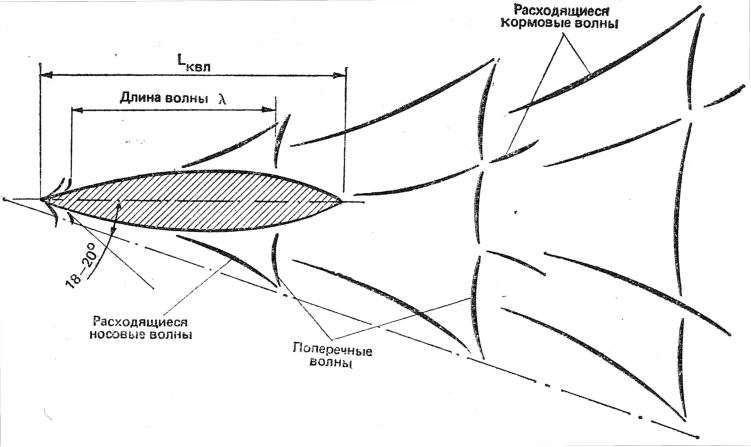
\includegraphics[scale=1.3]{0016P.pdf}
  \caption{Схема волновой системы, образующейся у корпуса судна}
  \label{fig:16}
\end{figure*}

Возникает сложная система носовых и кормовых волн, которая по своему характеру одинакова для судов любых размеров (рис.~\ris{16}). На малой скорости хорошо заметны расходящиеся волны, зарождающиеся в носу и корме судна. Их гребни расположены под углом 36\otdo 40\gr к диаметральной плоскости. На более высоких скоростях выделяются поперечные волны, гребни которые не выходят за пределы сектора, ограниченного углом 18\otdo 20\gr к \textit{ДП} судна. Носовая и кормовая системы поперечных волн взаимодействуют друг с другом, следствием чего может быть как увеличение высоты суммарной волны за кормой судна, так и её уменьшение. По мере удаления от судна энергия волн поглощается средой, и они постепенно затухают.

Величина волнового сопротивления изменяется в зависимости от скорости яхты. Из теории колебаний известно, что скорость распространения волн связана с их длиной $\lambda$ соотношением

\begin{equation}
  \lambda = \frac{2 \pi \cdot v^2}{\mathrm g}\,, \quad \text{м},
\end{equation}

где: $v$ \--- скорость яхты, м/с; $\mathrm g$ = 9,81 м/с$^2$ \--- ускорение силы тяжести. 

Поскольку волновая система движется вместе с яхтой, то и скорость распространения волны равна скорости яхты. Таким образом, можно подсчитать длину поперечной волны для каждой скорости яхты:

\begin{table*}[htb]
  \small
  \centering
  \begin{tabular}{l|c|c|c|c|c|c}
    \toprule
    Скорость, уз & 2 & 4 & 6 & 8 & 10 & 12 \\
    \midrule
    Длина волны, м & 0,68 & 2,72 & 6,12 & 10,9 & 17 & 24,5 \\
    \bottomrule
  \end{tabular}
  \caption{Зависимость длины поперечной волны от скорости яхты}
  \label{tab:1-2}
\end{table*}

Если речь идет, например, о яхте длиной по ватерлинии 8 м, то при скорости 4 уз на длине корпуса разместится около трех поперечных волн, при скорости 6 уз \--- полторы. Зависимость между длиной поперечной волны $\lambda$, создаваемой корпусом длиной \lkvl движущимся со скоростью $v$, во многом определяет величину волнового сопротивления. 

Для величины сопротивления важно, какая часть носовой поперечной волны подойдет к месту, где расположен гребень кормовой волны. Если на длине яхты по \textit{КВЛ} уложится целое число полуволн, то в корме может оказаться либо вершина, либо подошва носовой поперечной волны. Произойдет соответственно неблагоприятная (рис.~\ris{17}, \textit{б}) или благоприятная (рис.~\ris{17}, \textit{а}) интерференция волн. В первом случае высота суммарной волны возрастает и, поскольку энергия волн и величина волнового сопротивления пропорциональны квадрату их амплитуд, сопротивление яхты существенно возрастает. При благоприятном сложении подошвы носов волны с вершиной кормовой суммарная высота волны снизится, сопротивление увеличится медленнее.

\begin{figure*}[htb]
  \centering
  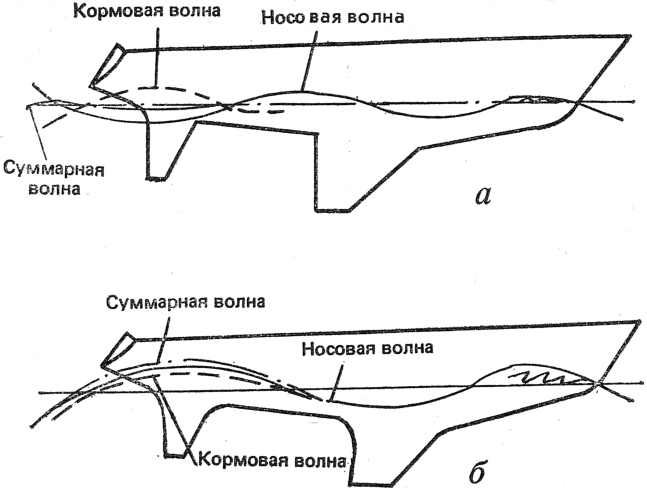
\includegraphics[scale=1.3]{0017P.pdf}
  \caption{Интерференция носовой и кормовой поперечных волн}
  \label{fig:17}
  \centering
  \small
  \textit{а} \--- благоприятная;
  \textit{б} \--- неблагоприятная
\end{figure*}

Многочисленными исследованиями, проведенными на моделях в опытном бассейне и на натурных судах, ycтановлено, что характер волнообразования всех судов, независимо от их размерений и абсолютной скорости, оказывается одинаков, если равны их относительные скорости или числа Фруда:

\begin{equation}
  \mathrm{Fr} = \frac{v}{(\mathrm g \cdot \lkvl)^{1/2}}
\end{equation}

Заметим, что в формулу относительной скорости входят длина судна по ватерлинии и те же символы, что и в формулу для определения длины волны в зависимости от её скорости. Этим подчеркивается взаимосвязь гравитационного характера волнообразования и его зависимость от скорости и длины судна.

На малых скоростях при $\mathrm{Fr} = 0,1\motdo 0,2$ волновое сопротивление яхты невелико. При $\mathrm{Fr} = 0,2$ на длине корпуса укладывается примерно четыре невысокие носовые поперечные волны. По мере повышения скорости волновое сопротивление начинает быстро расти. При числах Fr, равных 0,25, 0,30 и 0,50, имеет место неблагоприятная интерференция поперечных волн, а относительная скорость $\mathrm{Fr} = 0,5\motdo 0,6$ является порогом, превысить который обычная яхта водоизмещающего типа не может ни при каких обстоятельствах. На этой скорости яхта оказывается зажатой между двумя гребнями одной поперечной волны: сопротивление её возрастает пропорционально шестой степени скорости. Как правило, тяги парусов, даже при форсировании ими в свежий ветер, оказывается недостаточно, чтобы получить хотя бы небольшой прирост скорости. Поэтому скорость, соответствующую числу Фруда около 0,5, считают предельной для водоизмещающих яхт. Её можно вычислить, учитывая, что g \--- величина постоянная, по формуле\footnote{При переводе скорости из метрических мер в узлы и наоборот следует учитывать, что 1 узел = 1,852 км/ч = 0,514 м/с.}:

\begin{equation}
  v = 3 \cdot {\lkvl}^{1/2}, \quad \text{уз} 
\end{equation}

Таким образом, реальная скорость, которой могут достичь яхты отдельных типов, составляет около: 
\begin{itemize}
\item класс <<Солинг>> \--- 7,5 уз; 
\item тип <<Алькор>> \--- 9 уз; 
\item тип <<Конрад-54>> \--- 11,2 уз; 
\item класс R12 \--- 12 уз.
\end{itemize}

В ряде случаев в океанских гонках крейсерских яхт, однако, достигались более высокие скорости, которые могли развить в течение ограниченного времени суда облегченного типа. Это происходило, как правило, на попутных курсах и при крупной волне, при штормовых ветрах и форсировании парусами. В момент, когда под яхту подкатывался гребень очередной волны, смоченная поверхность корпуса резко уменьшалась и судно, выходило на режим серфинга \--- скольжения вместе с гребнем ветровой волны. При этом на яхте длиной по КВЛ 19,8 м, например, была отмечена максимальная скорость 22 уз ($v = 4,95 \cdot \lkvl$).

\begin{figure*}[htb]
  \centering
  \includegraphics[scale=1.3]{0018P.pdf}
  \caption{Зависимость сопротивления воды движению яхты от её скорости}
  \label{fig:18}
\end{figure*}

Как видно на рис.\ris{18}, доля волнового сопротивления в общем балансе сопротивления воды движению яхты возрастает с увеличением скорости яхты. На предельных скоростях оно достигает 60\otdo 65\,\%, а при движении в слабый ветер на создание волн затрачивается около 30\,\% движущей силы парусов. Поэтому снижение волнового сопротивления особенно важно для яхт, от которых ожидают хороших результатов в свежий ветер. При разработке проекта таких яхт стараются облегчить корпус и оборудование, чтобы значение относительной длины было в пределах $\lkvl / D^{1/3} = 4,2\motdo 5,2$ (чем больше эта длина, тем меньше волновое сопротивление). Коэффициент продольной полноты $\varphi$ принимают равным 0,60, чтобы более равномерно распределить водоизмещение яхты по длине и уменьшить глубину волновой впадины вблизи миделя.

Большое влияние на волновое сопротивление оказывает и отношение $\lkvl / \bkvl$. Благодаря большому удлинению корпусов катамаранов ($\lkvl / \bkvl = 10\motdo 20$) и отсутствию на них тяжелых фальшкилей удается существенно снизить их волновое сопротивление и достичь гораздо более высоких скоростей, чем $3 \cdot {\lkvl}^{1/2}$. Например, катамаран типа <<Центаурус>> ($\lkvl = 10$\,м) при благоприятных условиях развивает скорость 18 уз ($\approx 5,8 \cdot {\lkvl}^{1/2}$). 

\textbf{Дополнительное сопротивление на взволнованном море.} Нередко яхтсмены обнаруживают, что после многих часов, затраченных на лавировку против волны, яхта выбирается на ветер считанные мили. И это после изматывающей килевой качки! 

В данном случае приходится считаться с дополнительным сопротивлением движению яхты, которое появляется вследствие килевой качки судна. Особенно заметно падение скорости яхты, если период ее собственных продольных колебаний совпадает с периодом волны, т.\=,е. при резонансе. В существовании же собственных колебаний можно убедиться, если, например, спрыгнуть с носа яхты на причал. Каждая яхта при этом ведет себя, по-разному: у одной качка порывистая скоро затухает, у другой \--- плавная продолжается долго. 

Установлено, что период собственных продольных колебаний яхты зависит от продольного момента инерции т.\=,е. от расположения масс по длине судна, от обводов корпуса, особенно в оконечностях, взаимного расположения центра тяжести площади ватерлинии и центра тяжести яхты. Если, например, \textit{ЦТ} площади ватерлинии совпадает с \textit{ЦТ} яхты. Большие массы (якоря с цепями, двигатель цистерны топлива и пресной воды и т.\=,п.) расположены далеко от миделя и обводы, носа и кормы почти симметричны, яхта имеет достаточно большой период и амплитуду собственных колебаний, который может оказаться близким к периоду наиболее неблагоприятной волны длиной от 0,8 до 1,5 длины яхты по \textit{КВЛ}. При сильной килевой качке яхта приводит в движение большие массы воды, непосредственно соприкасающиеся с корпусом, таким образом, поглощается часть энергии ветра, которая могла бы затрачиваться на продвижение судна вперед, а сопротивление воды повышается 2\otdo 25 раза (по сравнению с тихой волны). 

При проектировании яхт обычно предусматривается возможность уменьшения размахов оконечностей яхты и смягчения качки. Наиболее тяжелые массы (фальшкиль, мачту, двигатель, цистерны и т.\=,п.) стараются расположить вблизи центра тяжести судна. Обводы корпуса выше ватерлинии обычно выполняются несимметричными относительно миделя. По мере движения кормы вниз ширина ватерлинии у транца и погружающийся объем корпуса прогрессивно увеличиваются, препятствуя глубокому погружению кормы в воду и поглощая энергию качки. Хороший развал надводного борта в носу также способствует снижению ускорений носовой части яхты при движении ее вниз.
 
Большое значение для уменьшения продольной качки имеет уменьшение массы рангоута и такелажа, поскольку момент инерции массы яхты складывается из произведения отдельных масс на квадраты отстояния их от \textit{ЦТ} судна. Таким образом, влияние на продольную качку килограмма массы на топе мачты, отстоящей от \textit{ЦТ} на 12\,м, аналогично грузу 70\,кг, расположенным на уровне палубы. 

Рис.~\ris{18} дает представление о доле добавочного сопротивления при ходе на волнении для крейсерско-гоночной яхты. При увеличении скорости эта составляющая общего сопротивления может возрасти до 15\otdo 25\,\%, что равносильно потере скорости на 3\otdo 4\,\%. Потеря существенно возрастает при резонансе, поэтому экипаж должен предпринять специальные меры для уменьшения амплитуды и изменения частоты колебаний. С этой целью можно изменить курс яхты по отношению к волне, если позволяют обстоятельства, или попытаться изменить период собственных колебаний судна, переместив людей на корму. Тогда яхта получит дифферент на корму, которая своим объемом и большой шириной ватерлинии будет гасить качку. 

\textbf{Дополнительное сопротивление от крена и дрейфа.} Испытания моделей яхт в опытных бассейнах показали, что с увеличением крена сопротивление корпуса превышает сопротивление тех же моделей, испытанных на ходу без крена. В качестве примера на рис.~\ris{18} дана кривая изменения дополнительного сопротивления яхты в зависимости от угла крена и скорости. При крене до 15\gr прирост сопротивления невелик \--- не более 5\,\%. Однако на скорости около 6 уз и при крене 35\gr сопротивление уже на 38\,\% больше, чем при плавании без крена. Для рассматриваемой яхты это приводит к потере 0,4 уз скорости. 

Эксперименты позволили выяснить, что дополнительное сопротивление в данном случае может быть разделено на две составляющие \--- индуктивное сопротивление и сопротивление от крена. Обе составляющие вызваны действием кренящей силы \vidx{F}{Д} (см. рис.~\ris{4}). Основным источником индуктивного сопротивления является подъемная сила на киле и руле, перетекание воды через нижнюю кромку плавников киля и руля со стороны повышенного давления на сторону разрежения, как мы уже говорили (см. рис.~\ris{20}). Срывающиеся с нижней кромки вихри требуют дополнительных затрат энергии движущей силы. Чем больше величина подъемной силы, образующейся на плавниках, тем больше разность давлений на их сторонах и соответственно больше индуктивное сопротивление. Наоборот, с увеличением аэродинамического удлинения плавника, т.\=,е. с уменьшением средней хорды относительно площади плавника, индуктивное сопротивление уменьшается. 

Определенную долю здесь вносит и корпус яхты, который обтекается не по оптимальным ватерлиниям, а под углом дрейфа. 

Дополнительное сопротивление от крена обусловлено как появлением несимметричности в обводах корпуса, так и изменением поля гидродинамических давлений у наветренного и подветренного бортов судна. У яхт с длинными свесами крен около 5\gr вызывает иногда даже некоторое снижение полного сопротивления при увеличении смоченной длины корпуса. Широкий <<швертботный>> современный корпус при крене 8\otdo 10\gr уменьшает смоченную поверхность и сопротивление, которое может снизиться на 2\otdo 4\,\%. Но с увеличением крена сопротивление начинает возрастать, составляя примерно 1/3 величины дополнительного сопротивления; остальное приходится на долю индуктивного сопротивления. И все же сопротивление от крена достаточно велико \--- оно достигает около 15\,\% сопротивления яхты, идущей без крена. Следовательно, при участии в гонке экипаж должен принять меры к уменьшению крена.

На рис.~\ris{18} хорошо видно, что крен 30\gr является для данной яхты критическим. Дальнейшее усиление ветра, при котором судно получает дополнительный крен, приводит уже не к повышению скорости, а, наоборот, к снижению. Значит, при достижении этого крена целесообразно уменьшить площадь парусности, а на небольшой яхте попытаться откренить судно массой экипажа.

При крене не только дополнительно растет сопротивление, но и ухудшается эффективность работы парусного вооружения, увеличивается склонность яхты приводиться к ветру. Для удержания судна на курсе необходимо отклонять руль на большой угол, что дополнительно увеличивает лобовое индуктивное сопротивление руля. 

Воздушное сопротивление корпуса яхты, рубок и экипажа, расположенного на палубе, сравнительно невелико. Оно достигает заметной величины только в сильный ветер и на курсе бейдевинд. Гораздо большее, значение имеет сопротивление рангоута, парусов и такелажа, рассмотрению которых уделено внимание в гл.~\ref{chap:2}.
